%\documentclass[preprint,3p,times,twocolumn]{elsarticle}
\documentclass[review,3p,times]{elsarticle}
\usepackage{amssymb}
\usepackage{amsmath}
\usepackage{graphicx}
\usepackage{bm}
\usepackage{yhmath}
\usepackage{subfigure}
\usepackage{multirow}
\usepackage{cleveref}
\usepackage{xcolor}
%\definecolor{Rv1}{rgb}{0,0,255}
\definecolor{Rv1}{rgb}{0,0,0}
%\definecolor{Rv2}{rgb}{0,0,255}
\definecolor{Rv2}{rgb}{0,0,0}
\usepackage{subdepth}
\usepackage[nomarkers,lists]{endfloat}

\def\pp#1#2{\frac{\partial #1}{\partial #2}}

\biboptions{comma,sort&compress}

\journal{Combustion and Flame}

\makeatletter
\def\@author#1{\g@addto@macro\elsauthors{\normalsize%
    \def\baselinestretch{1}%
    \upshape\authorsep#1\unskip\textsuperscript{%
      \ifx\@fnmark\@empty\else\unskip\sep\@fnmark\let\sep=,\fi
      \ifx\@corref\@empty\else\unskip\sep\@corref\let\sep=,\fi
      }%
    \def\authorsep{\unskip,\space}%
    \global\let\@fnmark\@empty
    \global\let\@corref\@empty  %% Added
    \global\let\sep\@empty}%
    \@eadauthor={#1}
}
\makeatother

\begin{document}

\begin{frontmatter}

\title{Stabilization of laminar nonpremixed DME/air coflow flames at elevated temperatures and pressures}

\author{Sili~Deng}
\author{Peng~Zhao}
\author{Michael E.~Mueller\corref{cor}}
\author{Chung K.~Law}
\cortext[cor]{Corresponding Author: muellerm@princeton.edu}

\address{Department of Mechanical and Aerospace Engineering, Princeton University, Princeton, NJ 08544, USA}

\begin{abstract}

The structure and stabilization mechanism of laminar nonpremixed autoignitive DME/air coflow flames were investigated at elevated temperatures and pressures. Computations with detailed chemistry were performed for DME and heated coflow air at $30$ atm with uniform inlet velocities ($2.4$, $3.2$, and $8.0$ m/s) imposed for both streams.  The heat release rate profiles are first examined for each case to demonstrate a multibrachial thermal structure.  Species concentrations and temperature were sampled along mixture fraction iso-contours, and Chemical Explosive Mode Analysis (CEMA) was performed to identify the controlling chemistry at representative points.  One-dimensional Lagrangian Flamelet Analysis (LFA) was also performed and compared with the two-dimensional computations to elucidate the relative importance of diffusion processes parallel and normal to the mixture fraction gradient.  Various coflow temperatures with different inlet velocities are examined to elucidate their influences on the multibrachial structure as well as the stabilization mechanism.  NTC (negative temperature coefficient)-affected inhomogeneous autoignition and the coupled effects with premixed flame propagation on stabilization are further studied.  It is found that, at high coflow boundary temperatures or low inlet velocities, the classical tribrachial flame structure is achieved, and autoignition contributes less to the stabilization due to reduced heat and radical accumulation.  The kinematic balance between the local flow speed and flame propagation speed is the dominant stabilization mechanism.  On the contrary, kinetic stabilization is achieved at lower coflow temperatures or higher inlet velocities as autoignition becomes dominant.  Due to the transition of the dominant chemical pathways during autoignition, the kinetically stabilized structure is usually multibrachial.  The transition of different stabilization mechanisms can be made by changing either the boundary velocity or temperature of the coflow.  Based on these results and previous work (Deng \emph{et al.} Combust. Flame 162 (2015) 3437-3445), a regime diagram is constructed that identifies the possible stabilization regimes: blow out, kinetically stabilized, autoignition-propagation-coupled stabilized, kinematically stabilized, and burner stabilized.          

\end{abstract}

\begin{keyword} 
Stabilization \sep Nonpremixed coflow flame \sep Autoignition \sep Negative temperature coefficient (NTC) \sep Dimethyl ether (DME) 
\end{keyword}

\end{frontmatter}


%\clearpage % For word count
%==============================================================

\section{Introduction}

%The stabilization of nonpremixed laminar lifted flames has been extensively investigated~\cite{chung07} at nonautoignitive conditions. A two-dimensional tribrachial structure (also known as triple flame)~\cite{buckmaster02} is observed.  Specifically, three branches, including a lean premixed flame wing, a rich premixed flame wing, and a trailing diffusion flame tail, intersect at a triple point, which is generally considered to be the stabilization point.  Under nonautoignitive conditions, the local flame propagation speed balances the incoming flow speed at the triple point, and this dynamic balance is considered to be the stabilization mechanism.  As reviewed by Chung~\cite{chung07}, burned gas expansion~\cite{ruetsch95,lee97,plessing98,kioni99}, concentration gradients~\cite{dold89,hartley91,ghosal00}, and velocity gradients~\cite{kim07} influence the local flame speed as well as the flow field, and, therefore, they also affect the stabilization, propagation, and instability of tribrachial flames.

\textcolor{Rv1}{Two-dimensional tribrachial structures (also known as triple flames)~\cite{buckmaster02} are observed in nonpremixed laminar lifted flames at nonautoignitive conditions.  The dynamic balance between the local flame propagation speed and the incoming flow speed at the triple point is generally considered as the stabilization mechanism~\cite{chung07}.}  However, practical engines operate at elevated pressures and temperatures.  As a consequence, the propensity for autoignition is significantly enhanced, and, therefore, the thermal and chemical structure of the tribrachial flame, as well as the stabilization mechanism, could be affected by the autoignition process.  \textcolor{Rv1}{For example, experimentally, Chung and co-workers have investigated autoignited lifted propane/nitrogen~\cite{choi09}, methane/hydrogen~\cite{choi12}, and other neat C$_1$ to C$_4$ hydrocarbon flames~\cite{choi10}, and compared their lift-off heights with homogeneous autoignition delay time.}  Furthermore, the autoignition process of most large hydrocarbons under practical engine conditions could possibly lie in the negative temperature coefficient (NTC) regime, in which the overall ignition delay time increases as the initial temperature increases.  The NTC phenomenon is relevant to engine knock~\cite{battin-leclerc08} and has been extensively studied in homogeneous systems~\cite{zador11}.  As Law and co-workers~\cite{law12,zhao13,deng14} recently demonstrated, ignition characteristics in a nonpremixed system can also be affected by NTC chemistry, especially at elevated pressures and/or extended residence times.  These computational and experimental studies were conducted in the nonpremixed counterflow system where the residence time is well characterized.  When the flow residence time and NTC chemistry timescales are comparable, the two processes are strongly coupled, resulting in modified system response, such as autoignition behavior.

To investigate autoignition with NTC chemistry effects in nonpremixed lifted flame stabilization, Krisman~\emph{et al.}~\cite{krisman14} recently conducted a numerical study of dimethyl ether (DME)/air nonpremixed flames at $40$ atmospheres and elevated air coflow temperatures ($700-1500$ K) and observed multibrachial thermal structures.  The autoignition response in the two-dimensional computation was compared with that of homogeneous autoignition under the same initial conditions.  A transport budget analysis of methoxymethylperoxy (CH$_3$OCH$_2$O$_2$) and hydroxyl (OH) radicals, which represent the low and high temperature chemistry, respectively, was performed to differentiate deflagration from autoignition.  The stabilization points of the multibrachial structure was determined with CH$_3$OCH$_2$O$_2$ and OH radical mass fractions for low and high temperature autoignition chemistry, respectively, and varied as boundary temperature and velocity changed.

More recently, to further elucidate the chemical structure of the multibrachial structure and the roles of autoignition and flame chemistry in the stabilization mechanism, the authors~\cite{deng15} performed a numerical study of nonpremixed DME/air coflow flames.  Chemical Explosive Mode Analysis (CEMA) was adopted to identify locally dominant reactions, and Lagrangian Flamelet Analysis (LFA) was adopted to identify the dominant combustion mode.  The comparison with the two-dimensional computation was able to quantify the relative importance of transport processes parallel and normal to the mixture fraction gradient and elucidate the dominant stabilization mechanism.  For increasing coflow boundary temperature at constant inlet velocities, the stabilization mechanism transitioned from kinetic to kinematic stabilization.

%In the present study, nonpremixed DME/air coflow flames at elevated temperatures and pressures were further studied.  As the previous work~\cite{deng15} focused on chemical effects on the stabilization by varying the coflow boundary temperature, the present study focuses on transport effects by changing the uniform inlet velocity at constant coflow temperature and in addition seeks to draw a complete regime diagram for the combined effects.  Moreover, NTC-affected inhomogeneous autoignition and its coupled effects with flame propagation on the stabilization are analyzed with CEMA and LFA.  

\textcolor{Rv1}{In the present study, nonpremixed DME/air coflow flames at elevated temperatures and pressures were further studied.  The objective of the current work is fourfold: first, to elucidate transport effects on stabilization, parallel to the previous work~\cite{deng15}, which focused on chemical effects; second, to demonstrate the effects of NTC chemistry on the multibrachial structure; third, to understand the transition between \emph{kinetic} and \emph{kinematic} stabilization mechanism and the coupling effects; and, fourth, to structure a complete regime diagram that includes both chemical and transport effects.}

\textcolor{Rv2}{As a final note, practical engine conditions are highly turbulent, and the autoignition phenomenon depends on both chemistry and turbulent mixing.  For example, in a DNS study, Yoo~\emph{et al.}~\cite{yoo11} observed the cyclic movement of the stabilization point of a turbulent lifted ethylene jet flame in highly-heated coflow, which is a consequence of consecutive autoignition events in the high-speed jet and coflow.  When fuels involve more complicated chemical characteristics, such as NTC effects, turbulence plays different and potentially competing roles. As demonstrated in a more recent computational work by Echekki and Ahmed~\cite{echekki15}, although scalar dissipation rate tends to delay ignition due to heat and radical loses from nascent kernels, enhanced mixing ensures much larger volumetric heat release rate after ignition.  However, neither of these works has considered high pressure regimes and analyzed the complicating effects of NTC in detail.  Therefore, in order to better understand flame stabilization and provide insights for future studies on turbulent lifted flames at elevated temperatures and pressures, the current work focuses on laminar conditions.}

 
%===============================================================

\section{Computational details} \label{sec:computation}

An axisymmetric DME stream at $300$ K is surrounded by heated coflow air at $30$ atmospheres.  The fuel nozzle diameter $D$ is $0.8$ mm, and the fuel and air are initially separated by an adiabatic, no-slip wall with thickness $D/20$.  The diameter of the coflow is $3.9$ mm with adiabatic, slip wall boundary conditions.  This diameter was chosen to be wide enough such that further widening of the domain did not influence the computational results.  Uniform inlet velocities of $2.4$, $3.2$, and $8.0$ m/s for both streams were specified.  The outlet boundary condition is a convective outflow, which is a Neumann condition at steady-state.

The governing equations, transport model, and chemical model were adopted to be the same as in Deng~\emph{et al.}~\cite{deng15}.  In brief, the Navier-Stokes equation with buoyancy effects in the streamwise direction and the conservation equations of mass, species, and energy were solved.  The species diffusivities are determined assuming a constant, nonunity Lewis number \textcolor{Rv1}{and kept the same as in the previous work~\cite{deng15}}.  The conserved scalar mixture fraction $Z$ is specified as unity and zero for the fuel stream and coflow, respectively, and is computed by solving a conserved scalar transport equation with unity Lewis number~\cite{pitsch98b}.  A DME skeletal mechanism of $39$ species~\cite{bhagatwala15}, which was reduced from the well-validated detailed mechanism of Zhao \emph{et al.}~\cite{zhao08}, was adopted as the chemical model.

The governing equations with the low-Mach number formulation are solved using NGA~\cite{desjardins08}.  The momentum and scalar equations are discretized with a second-order centered scheme and a third-order WENO scheme~\cite{liu94}, respectively, on a staggered mesh.  An iterative second-order semi-implicit Crank-Nicolson scheme is adopted for temporal integration~\cite{pierce01}.  The chemical source terms for the species and energy equations are integrated using the CVODE package~\cite{cohen96}.

Leveraging previous grid convergence studies~\cite{deng15}, uniform grid spacing in the axial direction was set to $\Delta x = 2.2-4.8$ ${\rm \mu}$m, depending on the case.  Nonuniform grid spacing in the radial direction was set to minimum $\Delta r = 2.5$ ${\rm \mu}$m to resolve the mixing layer near the thin wall, and the grid stretch rate was less than $3$\%.  Details about the numerical discretization are summarized in Table~\ref{table:domain_V}.      

%===============================================================

\section{Transport effects}

Transport effects on nonpremixed coflow flame stabilization were demonstrated by fixing the coflow temperature at $900$ K while varying the uniform inlet velocities as $2.4$, $3.2$, and $8.0$ m/s.  The $3.2$ m/s case was computed in previous work~\cite{deng15}.  

\begin{table*}
  \caption{Computational domain and number of grid points.}
  \label{table:domain_V}
  \centering
  \normalsize
  \resizebox{0.4\textwidth}{!}{
  \begin{tabular}{lc*{2}{c}}
    \hline
    Inlet Velocity [m/s]& $2.4$  & $3.2$  & $8.0$   \\
    \hline
    $L_x$ [mm]& $3.5$ & $3.5$ & $15$\\
    %Coflow O.D. [mm]& $3.9$ & $3.9$ & $3.9$\\
    $N_x$ & $1536$ & $1536$  & $3072$\\
    $N_r$ & $176$ & $176$ & $176$\\
    \hline
   \end{tabular}
}
\end{table*}

\subsection{Thermal and chemical structure}  
The heat release rate profiles for the three cases are shown in Fig.~\ref{fig:HRR_V}.  A qualitative determination of the stabilization point is the most upstream point on the largest heat release contour (the leading point), colored by red.  The mixture fraction iso-contours of $Z_{\rm st} = 0.1005$, $Z = 0.2$, and $Z = 0.3$ are delineated in solid black lines, from right to left.

When the inlet velocity is the lowest, $2.4$ m/s, a tribrachial thermal structure is observed very similar to that of the classical triple flame.  The triple point at $Z = 0.15$, where the three large heat release branches intersect, is also the stabilization point.  Some heat release can be found upstream of the tribrachial thermal structure for the partially reacting mixture at elevated temperature but is much less than the heat release from the flame structure.  As the inlet velocity increases to $3.2$ m/s, another branch with large heat release is found attached to the tribrachial structure around $Z = 0.2$.  The stabilization point is, again, the same as the triple point.  This structure has been analyzed in our previous work~\cite{deng15}.  However, as the inlet velocity further increases to $8.0$ m/s, the stabilization point is no longer on the tribrachial structure.  Instead, it is found to be near $Z = 0.25$ and is the intersection point of two trailing heat release branches.  Attached to the leaner branch, there is a tribrachial structure that appears similar to the triple flame structure.  This multibrachial structure is similar to the one found in previous work at a higher oxidizer temperature ($800$ K) but lower velocity ($3.2$ m/s)~\cite{deng15}.

\begin{figure}[t]
  \centering
  \scriptsize
  \vspace{-0.1in}
  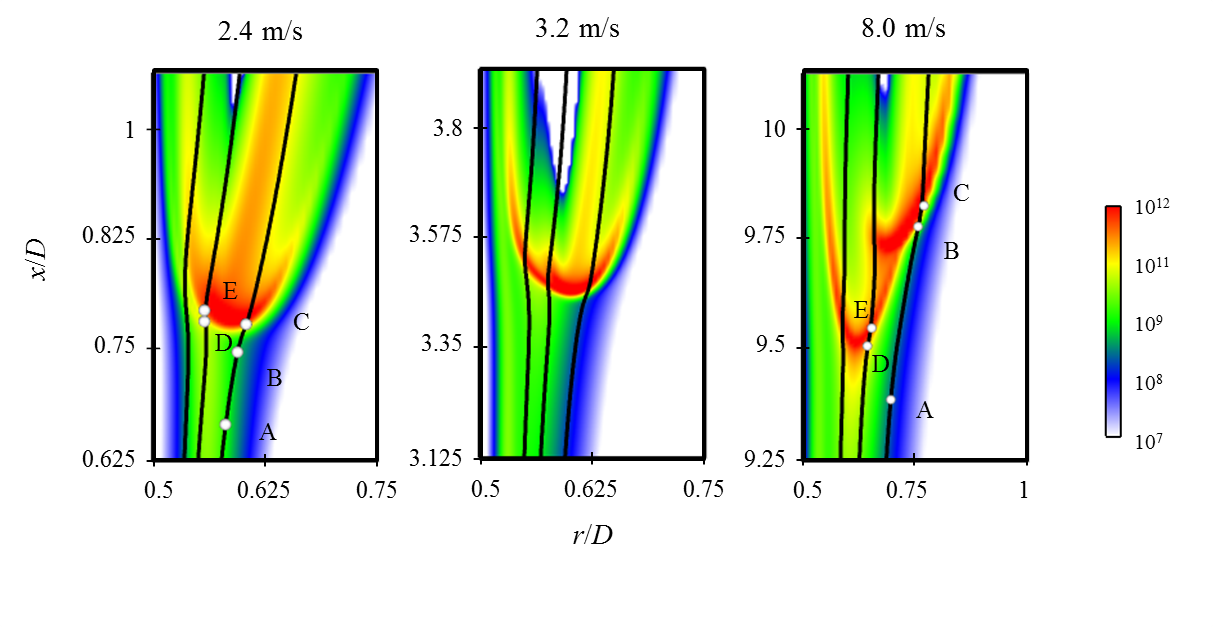
\includegraphics[width=0.7\textwidth]{HRR_V.png}
  \normalsize
  \vspace{-0.4in}
  \caption{Heat release rate [J/m$^3$-s] profiles.  The iso-contours of $Z_{\rm st}$, $Z = 0.2$, and $Z = 0.3$ are outlined from right to left in solid lines, respectively.  The CEMA sampling points for $2.4$ and $8.0$ m/s cases are marked along the iso-contours.}
  \label{fig:HRR_V}
\end{figure}

The controlling chemistry of the three cases was studied with CEMA~\cite{lu10,shan12}.   Briefly, local species concentrations and temperature are sampled from the two-dimensional computation and input into CEMA to evaluate the eigenvalues of the Jacobian matrix ($K + 1$ by $K + 1$, where $K$ is the number of species) of the chemical source terms.  The eigenmode associated with the eigenvalue $\lambda_{\rm e}$, which has the largest real part among all the eigenvalues, is defined as a chemical explosive mode, if

\begin{equation}
\rm{Re}(\lambda_{\rm e}) > 0, \lambda_{\rm e} = \mathbf{b_{\rm e}J_{\omega}a_{\rm e}},
\end{equation}
where $\mathbf{b_{\rm e}}$ and $\mathbf{a_{\rm e}}$ are the left and right eigenvectors, respectively, associated with $\lambda_{\rm e}$, and $\mathbf{J_{\omega}}$ is the chemical Jacobian matrix.  The existence of the chemical explosive mode indicates the propensity of local mixture autoignition given an isolated, adiabatic, and constant volume environment.  Furthermore, the detailed chemical reactions that contribute to the chemical explosive mode can be quantified by the explosion participation index:

\begin{equation}
\mathbf{PI} = \frac{|(\mathbf{b_{\rm e}} \cdot \mathbf{S}) \otimes \mathbf{R}|}{sum(|(\mathbf{b_{\rm e}} \cdot \mathbf{S}) \otimes \mathbf{R}|)},
\end{equation}
where $\mathbf{S}$ is the stoichiometric coefficient matrix, $\mathbf{R}$ is the vector of the net rates for the reactions, and $\otimes$ denotes elementwise multiplication of two vectors.  

In the present study, such samplings were conducted along $Z_{\rm st}$, $Z = 0.2$, and $Z = 0.3$ iso-contours, as shown in Fig.~\ref{fig:HRR_V}.  Based on the explosive mode and participation index, the evolution of the dominant reactions is shown in Fig.~\ref{fig:CEMA_V}.

\begin{figure}
  \centering
  \scriptsize
  \resizebox{1.0\textwidth}{!}{% GNUPLOT: LaTeX picture with Postscript
\begingroup
  \makeatletter
  \providecommand\color[2][]{%
    \GenericError{(gnuplot) \space\space\space\@spaces}{%
      Package color not loaded in conjunction with
      terminal option `colourtext'%
    }{See the gnuplot documentation for explanation.%
    }{Either use 'blacktext' in gnuplot or load the package
      color.sty in LaTeX.}%
    \renewcommand\color[2][]{}%
  }%
  \providecommand\includegraphics[2][]{%
    \GenericError{(gnuplot) \space\space\space\@spaces}{%
      Package graphicx or graphics not loaded%
    }{See the gnuplot documentation for explanation.%
    }{The gnuplot epslatex terminal needs graphicx.sty or graphics.sty.}%
    \renewcommand\includegraphics[2][]{}%
  }%
  \providecommand\rotatebox[2]{#2}%
  \@ifundefined{ifGPcolor}{%
    \newif\ifGPcolor
    \GPcolortrue
  }{}%
  \@ifundefined{ifGPblacktext}{%
    \newif\ifGPblacktext
    \GPblacktexttrue
  }{}%
  % define a \g@addto@macro without @ in the name:
  \let\gplgaddtomacro\g@addto@macro
  % define empty templates for all commands taking text:
  \gdef\gplbacktext{}%
  \gdef\gplfronttext{}%
  \makeatother
  \ifGPblacktext
    % no textcolor at all
    \def\colorrgb#1{}%
    \def\colorgray#1{}%
  \else
    % gray or color?
    \ifGPcolor
      \def\colorrgb#1{\color[rgb]{#1}}%
      \def\colorgray#1{\color[gray]{#1}}%
      \expandafter\def\csname LTw\endcsname{\color{white}}%
      \expandafter\def\csname LTb\endcsname{\color{black}}%
      \expandafter\def\csname LTa\endcsname{\color{black}}%
      \expandafter\def\csname LT0\endcsname{\color[rgb]{1,0,0}}%
      \expandafter\def\csname LT1\endcsname{\color[rgb]{0,1,0}}%
      \expandafter\def\csname LT2\endcsname{\color[rgb]{0,0,1}}%
      \expandafter\def\csname LT3\endcsname{\color[rgb]{1,0,1}}%
      \expandafter\def\csname LT4\endcsname{\color[rgb]{0,1,1}}%
      \expandafter\def\csname LT5\endcsname{\color[rgb]{1,1,0}}%
      \expandafter\def\csname LT6\endcsname{\color[rgb]{0,0,0}}%
      \expandafter\def\csname LT7\endcsname{\color[rgb]{1,0.3,0}}%
      \expandafter\def\csname LT8\endcsname{\color[rgb]{0.5,0.5,0.5}}%
    \else
      % gray
      \def\colorrgb#1{\color{black}}%
      \def\colorgray#1{\color[gray]{#1}}%
      \expandafter\def\csname LTw\endcsname{\color{white}}%
      \expandafter\def\csname LTb\endcsname{\color{black}}%
      \expandafter\def\csname LTa\endcsname{\color{black}}%
      \expandafter\def\csname LT0\endcsname{\color{black}}%
      \expandafter\def\csname LT1\endcsname{\color{black}}%
      \expandafter\def\csname LT2\endcsname{\color{black}}%
      \expandafter\def\csname LT3\endcsname{\color{black}}%
      \expandafter\def\csname LT4\endcsname{\color{black}}%
      \expandafter\def\csname LT5\endcsname{\color{black}}%
      \expandafter\def\csname LT6\endcsname{\color{black}}%
      \expandafter\def\csname LT7\endcsname{\color{black}}%
      \expandafter\def\csname LT8\endcsname{\color{black}}%
    \fi
  \fi
  \setlength{\unitlength}{0.0500bp}%
  \begin{picture}(7200.00,5040.00)%
    \gplgaddtomacro\gplbacktext{%
      \csname LTb\endcsname%
      \put(2748,1043){\makebox(0,0)[r]{\strut{}CH$_3$OCH$_2$+O$_2$$\Longleftrightarrow$CH$_3$OCH$_2$O$_2$}}%
      \put(2748,1383){\makebox(0,0)[r]{\strut{}CH$_2$OCH$_2$O$_2$H$\Longleftrightarrow$OH+CH$_2$O+CH$_2$O}}%
      \put(2748,1722){\makebox(0,0)[r]{\strut{}CH$_3$OCH$_3$+OH$\Longleftrightarrow$CH$_3$OCH$_2$+H$_2$O}}%
      \put(2748,2061){\makebox(0,0)[r]{\strut{}H+O$_2$+M$\Longleftrightarrow$HO$_2$+M}}%
      \put(2748,2400){\makebox(0,0)[r]{\strut{}HCO+O$_2$$\Longleftrightarrow$CO+HO$_2$}}%
      \put(2748,2740){\makebox(0,0)[r]{\strut{}CH$_3$OCH$_2$O$_2$$\Longleftrightarrow$CH$_2$OCH$_2$O$_2$H}}%
      \put(2748,3079){\makebox(0,0)[r]{\strut{}CH$_2$O+OH$\Longleftrightarrow$HCO+H$_2$O}}%
      \put(2748,3418){\makebox(0,0)[r]{\strut{}HO$_2$CH$_2$OCHO$\Longleftrightarrow$OCH$_2$OCHO+OH}}%
      \put(2748,3757){\makebox(0,0)[r]{\strut{}CH$_2$O+H$\Longleftrightarrow$HCO+H$_2$}}%
      \put(2748,4097){\makebox(0,0)[r]{\strut{}CH$_3$OCH$_3$+H$\Longleftrightarrow$CH$_3$OCH$_2$+H$_2$}}%
      \put(2748,4436){\makebox(0,0)[r]{\strut{}H+O$_2$$\Longleftrightarrow$O+OH}}%
      \put(2880,484){\makebox(0,0){\strut{}-1}}%
      \put(3861,484){\makebox(0,0){\strut{}-0.5}}%
      \put(4842,484){\makebox(0,0){\strut{} 0}}%
      \put(5822,484){\makebox(0,0){\strut{} 0.5}}%
      \put(6803,484){\makebox(0,0){\strut{} 1}}%
      \csname LTb\endcsname%
      \put(4841,154){\makebox(0,0){\strut{}Normalized Participation Index}}%
      \put(5234,1332){\makebox(0,0)[l]{\strut{}Point A}}%
      \put(5234,1501){\makebox(0,0)[l]{\strut{}Point B}}%
      \put(5234,1688){\makebox(0,0)[l]{\strut{}Point C}}%
      \put(5234,1857){\makebox(0,0)[l]{\strut{}Point D}}%
      \put(5234,2027){\makebox(0,0)[l]{\strut{}Point E}}%
      \put(5234,2231){\makebox(0,0)[l]{\strut{}$2.4$ m/s}}%
    }%
    \gplgaddtomacro\gplfronttext{%
      \csname LTb\endcsname%
      \put(5690,1337){\makebox(0,0)[r]{\strut{} }}%
      \csname LTb\endcsname%
      \put(5690,1513){\makebox(0,0)[r]{\strut{} }}%
      \csname LTb\endcsname%
      \put(5690,1689){\makebox(0,0)[r]{\strut{} }}%
      \csname LTb\endcsname%
      \put(5690,1865){\makebox(0,0)[r]{\strut{} }}%
      \csname LTb\endcsname%
      \put(5690,2041){\makebox(0,0)[r]{\strut{} }}%
    }%
    \gplbacktext
    \put(0,0){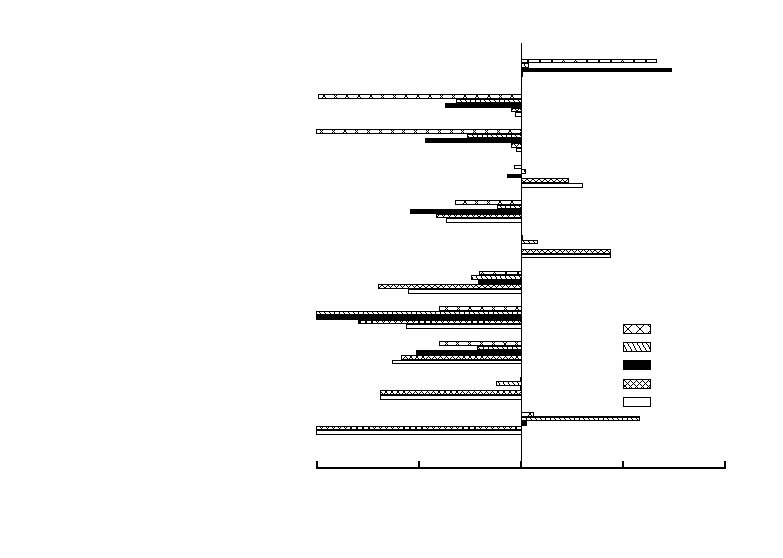
\includegraphics{ch-dynamics/CEMA_24}}%
    \gplfronttext
  \end{picture}%
\endgroup
}
  \resizebox{1.0\textwidth}{!}{% GNUPLOT: LaTeX picture with Postscript
\begingroup
  \makeatletter
  \providecommand\color[2][]{%
    \GenericError{(gnuplot) \space\space\space\@spaces}{%
      Package color not loaded in conjunction with
      terminal option `colourtext'%
    }{See the gnuplot documentation for explanation.%
    }{Either use 'blacktext' in gnuplot or load the package
      color.sty in LaTeX.}%
    \renewcommand\color[2][]{}%
  }%
  \providecommand\includegraphics[2][]{%
    \GenericError{(gnuplot) \space\space\space\@spaces}{%
      Package graphicx or graphics not loaded%
    }{See the gnuplot documentation for explanation.%
    }{The gnuplot epslatex terminal needs graphicx.sty or graphics.sty.}%
    \renewcommand\includegraphics[2][]{}%
  }%
  \providecommand\rotatebox[2]{#2}%
  \@ifundefined{ifGPcolor}{%
    \newif\ifGPcolor
    \GPcolortrue
  }{}%
  \@ifundefined{ifGPblacktext}{%
    \newif\ifGPblacktext
    \GPblacktexttrue
  }{}%
  % define a \g@addto@macro without @ in the name:
  \let\gplgaddtomacro\g@addto@macro
  % define empty templates for all commands taking text:
  \gdef\gplbacktext{}%
  \gdef\gplfronttext{}%
  \makeatother
  \ifGPblacktext
    % no textcolor at all
    \def\colorrgb#1{}%
    \def\colorgray#1{}%
  \else
    % gray or color?
    \ifGPcolor
      \def\colorrgb#1{\color[rgb]{#1}}%
      \def\colorgray#1{\color[gray]{#1}}%
      \expandafter\def\csname LTw\endcsname{\color{white}}%
      \expandafter\def\csname LTb\endcsname{\color{black}}%
      \expandafter\def\csname LTa\endcsname{\color{black}}%
      \expandafter\def\csname LT0\endcsname{\color[rgb]{1,0,0}}%
      \expandafter\def\csname LT1\endcsname{\color[rgb]{0,1,0}}%
      \expandafter\def\csname LT2\endcsname{\color[rgb]{0,0,1}}%
      \expandafter\def\csname LT3\endcsname{\color[rgb]{1,0,1}}%
      \expandafter\def\csname LT4\endcsname{\color[rgb]{0,1,1}}%
      \expandafter\def\csname LT5\endcsname{\color[rgb]{1,1,0}}%
      \expandafter\def\csname LT6\endcsname{\color[rgb]{0,0,0}}%
      \expandafter\def\csname LT7\endcsname{\color[rgb]{1,0.3,0}}%
      \expandafter\def\csname LT8\endcsname{\color[rgb]{0.5,0.5,0.5}}%
    \else
      % gray
      \def\colorrgb#1{\color{black}}%
      \def\colorgray#1{\color[gray]{#1}}%
      \expandafter\def\csname LTw\endcsname{\color{white}}%
      \expandafter\def\csname LTb\endcsname{\color{black}}%
      \expandafter\def\csname LTa\endcsname{\color{black}}%
      \expandafter\def\csname LT0\endcsname{\color{black}}%
      \expandafter\def\csname LT1\endcsname{\color{black}}%
      \expandafter\def\csname LT2\endcsname{\color{black}}%
      \expandafter\def\csname LT3\endcsname{\color{black}}%
      \expandafter\def\csname LT4\endcsname{\color{black}}%
      \expandafter\def\csname LT5\endcsname{\color{black}}%
      \expandafter\def\csname LT6\endcsname{\color{black}}%
      \expandafter\def\csname LT7\endcsname{\color{black}}%
      \expandafter\def\csname LT8\endcsname{\color{black}}%
    \fi
  \fi
  \setlength{\unitlength}{0.0500bp}%
  \begin{picture}(7200.00,5040.00)%
    \gplgaddtomacro\gplbacktext{%
      \csname LTb\endcsname%
      \put(2748,1043){\makebox(0,0)[r]{\strut{}H$_2$O$_2$+M$\Longleftrightarrow$OH+OH+M}}%
      \put(2748,1383){\makebox(0,0)[r]{\strut{}HCO+O$_2$$\Longleftrightarrow$CO+HO$_2$}}%
      \put(2748,1722){\makebox(0,0)[r]{\strut{}CH$_2$O+OH$\Longleftrightarrow$HCO+H$_2$O}}%
      \put(2748,2061){\makebox(0,0)[r]{\strut{}HO$_2$+HO$_2$$\Longleftrightarrow$H$_2$O$_2$+O$_2$}}%
      \put(2748,2400){\makebox(0,0)[r]{\strut{}CH$_3$OCH$_3$+HO$_2$$\Longleftrightarrow$CH$_3$OCH$_2$+H$_2$O$_2$}}%
      \put(2748,2740){\makebox(0,0)[r]{\strut{}CH$_3$OCH$_2$O$_2$$\Longleftrightarrow$CH$_2$OCH$_2$O$_2$H}}%
      \put(2748,3079){\makebox(0,0)[r]{\strut{}CH$_2$OCH$_2$O$_2$H$\Longleftrightarrow$OH+CH$_2$O+CH$_2$O}}%
      \put(2748,3418){\makebox(0,0)[r]{\strut{}CH$_3$OCH$_2$+O$_2$$\Longleftrightarrow$CH$_3$OCH$_2$O$_2$}}%
      \put(2748,3757){\makebox(0,0)[r]{\strut{}CH$_2$O+HO$_2$$\Longleftrightarrow$HCO+H$_2$O$_2$}}%
      \put(2748,4097){\makebox(0,0)[r]{\strut{}H+O$_2$+M$\Longleftrightarrow$HO$_2$+M}}%
      \put(2748,4436){\makebox(0,0)[r]{\strut{}H+O$_2$$\Longleftrightarrow$O+OH}}%
      \put(2880,484){\makebox(0,0){\strut{}-1}}%
      \put(3861,484){\makebox(0,0){\strut{}-0.5}}%
      \put(4842,484){\makebox(0,0){\strut{} 0}}%
      \put(5822,484){\makebox(0,0){\strut{} 0.5}}%
      \put(6803,484){\makebox(0,0){\strut{} 1}}%
      \csname LTb\endcsname%
      \put(4841,154){\makebox(0,0){\strut{}Normalized Participation Index}}%
      \put(5234,1332){\makebox(0,0)[l]{\strut{}Point A}}%
      \put(5234,1501){\makebox(0,0)[l]{\strut{}Point B}}%
      \put(5234,1688){\makebox(0,0)[l]{\strut{}Point C}}%
      \put(5234,1857){\makebox(0,0)[l]{\strut{}Point D}}%
      \put(5234,2027){\makebox(0,0)[l]{\strut{}Point E}}%
      \put(5234,2231){\makebox(0,0)[l]{\strut{}$8.0$ m/s}}%
    }%
    \gplgaddtomacro\gplfronttext{%
      \csname LTb\endcsname%
      \put(5690,1337){\makebox(0,0)[r]{\strut{} }}%
      \csname LTb\endcsname%
      \put(5690,1513){\makebox(0,0)[r]{\strut{} }}%
      \csname LTb\endcsname%
      \put(5690,1689){\makebox(0,0)[r]{\strut{} }}%
      \csname LTb\endcsname%
      \put(5690,1865){\makebox(0,0)[r]{\strut{} }}%
      \csname LTb\endcsname%
      \put(5690,2041){\makebox(0,0)[r]{\strut{} }}%
    }%
    \gplbacktext
    \put(0,0){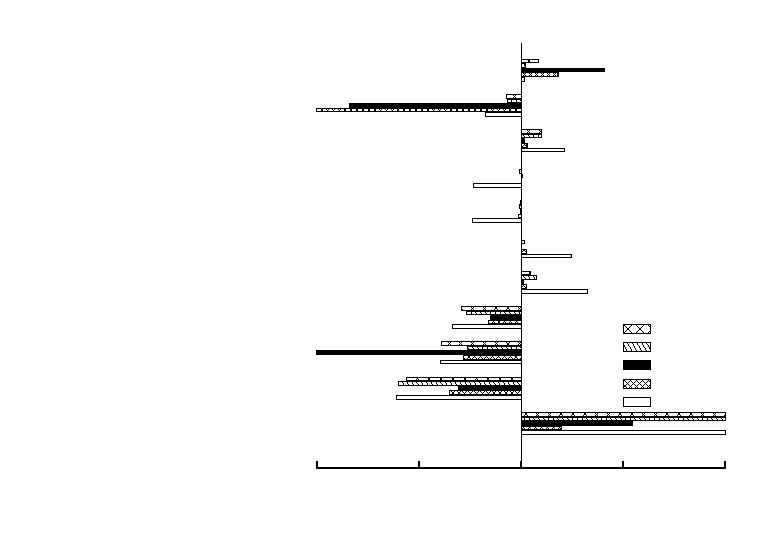
\includegraphics{ch-dynamics/CEMA_80}}%
    \gplfronttext
  \end{picture}%
\endgroup
}
  \normalsize
  \caption{Normalized participation index at $2.4$ and $8.0$ m/s.  Sampled locations are delineated in Fig.~\ref{fig:HRR_V}.}
  \label{fig:CEMA_V}
\end{figure}

At $2.4$ m/s, the dominant reactions along $Z_{\rm st}$ and $Z = 0.2$ iso-contours evolve in similar ways: upstream of the tribrachial structure (points A, B, and D), low temperature chemistry, characterized by reactions involving CH$_3$OCH$_2$O$_2$ radicals, is active.  Due to the high diffusivity of H radicals and the elevated pressure, the H radical recombination reaction (H + O$_2$ + M $\Longleftrightarrow$ HO$_2$ + M) is important.  At the most reactive region (points C and E), the H radical branching reaction (H + O$_2$ $\Longleftrightarrow$ O + OH) becomes the most important chain branching reaction, indicating the transition to high temperature chemistry.  On the contrary, for the $8.0$ m/s case, while low temperature chemistry is still active upstream of the multibrachial structure, the dominant chain branching reaction is the hydrogen peroxide branching reaction (H$_2$O$_2$ + M $\Longleftrightarrow$ OH + OH + M).  Moreover, the dominant reactions along the $Z_{\rm st}$ and $Z = 0.2$ iso-contours evolve in different ways.  Along the $Z = 0.2$ iso-contour, from point D to E, the hydrogen peroxide branching reaction is always the dominant reaction, indicating the role of low-to-intermediate temperature autoignition chemistry~\cite{westbrook00}.  Although this is the case at point A on the $Z_{\rm st}$ iso-contour, the H radical chain branching reaction becomes dominant at point C, the most reactive zone, indicating that the dominant chemical pathway shifts to high temperature chemistry.  CEMA results for the $3.2$ m/s case show similar transitions as those of the $8.0$ m/s case, although their thermal structures appear different.  Therefore, further computational diagnostics is needed to identify the dominant combustion mode.   

\subsection{Stabilization mechanism} 
The above CEMA results have demonstrated the importance of autoignition chemistry in the multibrachial structure.  However, further analysis is still needed to elucidate the role that autoignition plays in the stabilization mechanism.  As conducted previously~\cite{deng15}, LFA~\cite{pitsch98a} utilizes the initial conditions provided by the two-dimensional computation to provide the time history of the one-dimensional inhomogeneous autoignition.  As only the diffusion processes parallel to the mixture fraction gradient direction are accounted for in this analysis, the comparison of this one-dimensional flamelet and the two-dimensional result gives the relative importance of transport parallel and normal to the mixture fraction gradient and thus the relative importance of inhomogeneous autoignition and premixed flame propagation to the stabilization mechanism.

Specifically, the unsteady flamelets were computed with FlameMaster~\cite{flamemaster}.  Species mass fractions and temperature were sampled at ten times the wall thickness downstream of the inlet to avoid the influence from the recirculation zone (behind the thin wall) on the initial condition in LFA.  The time history of the scalar dissipation rate was sampled along the $Z_{\rm st}$ iso-contour from the two-dimensional computation.  The flamelet time was computed from the two-dimensional computational results, along the $Z_{\rm st}$ iso-contour: 
 \begin{equation} \label{eq:t}
t = \int ^{x}_{0} \frac{1}{(u + u_Z)(x')|(Z=Z_{\rm st})} dx'.
\end{equation} 
The axial component of the mixture fraction iso-contour propagation speed relative to the fluid convection $u_Z$ is taken into consideration in addition to the axial component of the fluid convection velocity $u$.  The expression for $u_Z$ is adopted from Lignell \emph {et al.}~\cite{lignell07}:
\begin{equation}
\mathbf{u_Z} = -\frac{\nabla \cdot (\rho D_Z \nabla Z) }{\rho |\nabla Z|} \mathbf{n},
\end{equation}
where $D_Z$ is the mixture fraction diffusivity, with unity Lewis number, and $\rho$ is the density.  The normal vector \textbf{n}, defined as
\begin{equation}
\mathbf{n} = \frac{\nabla Z}{|\nabla Z|},
\end{equation}
indicates the direction of this diffusion induced relative velocity.  Only the scalar dissipation rate at stoichiometric mixture fraction is sampled from the two-dimensional computations; the dissipation rates at other mixture fractions were computed assuming the following form~\cite{petersbook}:
\begin{equation} \label{eq:Zref}
\chi{(Z)} = \chi{(Z_{\rm st})} \frac{\exp{(-2[{\rm erfc}^{-1}(2Z)]^2)}}{\exp{(-2[{\rm erfc}^{-1}(2Z_{\rm st})]^2)}} = \chi{(Z_{\rm st})} f(Z;Z_{\rm st}).
\end{equation}
Validation of this expression was provided in previous work~\cite{deng15}.

The Lagrangian time history profiles of the two-dimensional computation and one-dimensional LFA are shown in Fig.~\ref{fig:LFA_V}.  For each inlet velocity case, the temperature profiles are compared along $Z_{\rm st}$, $Z = 0.2$, and $Z = 0.3$.

For the $2.4$ m/s case, LFA fails to match the two-dimensional result at all three mixture fractions, indicating that transport processes normal to the mixture fraction gradient are crucial, which further indicates that flame propagation is the dominant stabilization mechanism.  At $3.2$ m/s, LFA slightly lags behind the two-dimensional result at $Z_{\rm st}$ but matches well at $Z = 0.2$ and $Z = 0.3$.  Recalling the heat release profile in Fig.~\ref{fig:HRR_V}, these results indicate that the tetrabrachial structure consists of a tribrachial structure, at which flame propagation is not negligible, and the richer branch that intersects with the tribrachial flame is an autoignition front, whose response is well captured with the one-dimensional flamelet model.  As a result, stabilization of the $3.2$ m/s case is characterized as a mixed mode of inhomogeneous autoignition and premixed flame propagation, depending on the local mixture fraction.  At $8.0$ m/s, LFA agrees well with the two-dimensional result at all mixture fractions, indicating that the transport processes normal to the mixture fraction gradient are negligible.  Therefore, the stabilization mechanism is characterized as inhomogeneous autoignition.

\begin{figure}
  \centering
  \scriptsize
  \resizebox{1.0\textwidth}{!}{% GNUPLOT: LaTeX picture with Postscript
\begingroup
  \makeatletter
  \providecommand\color[2][]{%
    \GenericError{(gnuplot) \space\space\space\@spaces}{%
      Package color not loaded in conjunction with
      terminal option `colourtext'%
    }{See the gnuplot documentation for explanation.%
    }{Either use 'blacktext' in gnuplot or load the package
      color.sty in LaTeX.}%
    \renewcommand\color[2][]{}%
  }%
  \providecommand\includegraphics[2][]{%
    \GenericError{(gnuplot) \space\space\space\@spaces}{%
      Package graphicx or graphics not loaded%
    }{See the gnuplot documentation for explanation.%
    }{The gnuplot epslatex terminal needs graphicx.sty or graphics.sty.}%
    \renewcommand\includegraphics[2][]{}%
  }%
  \providecommand\rotatebox[2]{#2}%
  \@ifundefined{ifGPcolor}{%
    \newif\ifGPcolor
    \GPcolortrue
  }{}%
  \@ifundefined{ifGPblacktext}{%
    \newif\ifGPblacktext
    \GPblacktexttrue
  }{}%
  % define a \g@addto@macro without @ in the name:
  \let\gplgaddtomacro\g@addto@macro
  % define empty templates for all commands taking text:
  \gdef\gplbacktext{}%
  \gdef\gplfronttext{}%
  \makeatother
  \ifGPblacktext
    % no textcolor at all
    \def\colorrgb#1{}%
    \def\colorgray#1{}%
  \else
    % gray or color?
    \ifGPcolor
      \def\colorrgb#1{\color[rgb]{#1}}%
      \def\colorgray#1{\color[gray]{#1}}%
      \expandafter\def\csname LTw\endcsname{\color{white}}%
      \expandafter\def\csname LTb\endcsname{\color{black}}%
      \expandafter\def\csname LTa\endcsname{\color{black}}%
      \expandafter\def\csname LT0\endcsname{\color[rgb]{1,0,0}}%
      \expandafter\def\csname LT1\endcsname{\color[rgb]{0,1,0}}%
      \expandafter\def\csname LT2\endcsname{\color[rgb]{0,0,1}}%
      \expandafter\def\csname LT3\endcsname{\color[rgb]{1,0,1}}%
      \expandafter\def\csname LT4\endcsname{\color[rgb]{0,1,1}}%
      \expandafter\def\csname LT5\endcsname{\color[rgb]{1,1,0}}%
      \expandafter\def\csname LT6\endcsname{\color[rgb]{0,0,0}}%
      \expandafter\def\csname LT7\endcsname{\color[rgb]{1,0.3,0}}%
      \expandafter\def\csname LT8\endcsname{\color[rgb]{0.5,0.5,0.5}}%
    \else
      % gray
      \def\colorrgb#1{\color{black}}%
      \def\colorgray#1{\color[gray]{#1}}%
      \expandafter\def\csname LTw\endcsname{\color{white}}%
      \expandafter\def\csname LTb\endcsname{\color{black}}%
      \expandafter\def\csname LTa\endcsname{\color{black}}%
      \expandafter\def\csname LT0\endcsname{\color{black}}%
      \expandafter\def\csname LT1\endcsname{\color{black}}%
      \expandafter\def\csname LT2\endcsname{\color{black}}%
      \expandafter\def\csname LT3\endcsname{\color{black}}%
      \expandafter\def\csname LT4\endcsname{\color{black}}%
      \expandafter\def\csname LT5\endcsname{\color{black}}%
      \expandafter\def\csname LT6\endcsname{\color{black}}%
      \expandafter\def\csname LT7\endcsname{\color{black}}%
      \expandafter\def\csname LT8\endcsname{\color{black}}%
    \fi
  \fi
  \setlength{\unitlength}{0.0500bp}%
  \begin{picture}(8640.00,6048.00)%
    \gplgaddtomacro\gplbacktext{%
      \csname LTb\endcsname%
      \put(6694,4756){\makebox(0,0)[r]{\strut{} 800}}%
      \put(6694,4961){\makebox(0,0)[r]{\strut{} 1200}}%
      \put(6694,5167){\makebox(0,0)[r]{\strut{} 1600}}%
      \put(6694,5372){\makebox(0,0)[r]{\strut{} 2000}}%
      \put(6694,5578){\makebox(0,0)[r]{\strut{} 2400}}%
      \put(6694,5783){\makebox(0,0)[r]{\strut{} 2800}}%
      \put(6826,4536){\makebox(0,0){\strut{} 0}}%
      \put(7137,4536){\makebox(0,0){\strut{} 0.5}}%
      \put(7448,4536){\makebox(0,0){\strut{} 1}}%
      \put(7759,4536){\makebox(0,0){\strut{} 1.5}}%
      \put(8070,4536){\makebox(0,0){\strut{} 2}}%
      \put(5792,5269){\rotatebox{-270}{\makebox(0,0){\strut{}\vspace{-36pt}$T$ [K]}}}%
      \put(7448,4206){\makebox(0,0){\strut{}\vspace{12pt}Time [ms]}}%
      \put(1987,6047){\makebox(0,0)[l]{\strut{}$2.4$ m/s}}%
      \put(4579,6047){\makebox(0,0)[l]{\strut{}$3.2$ m/s}}%
      \put(7170,6047){\makebox(0,0)[l]{\strut{}$8.0$ m/s}}%
      \put(-172,1633){\makebox(0,0)[l]{\strut{}$Z = 0.3$}}%
      \put(-172,3447){\makebox(0,0)[l]{\strut{}$Z = 0.2$}}%
      \put(-172,5261){\makebox(0,0)[l]{\strut{}$Z = Z_{\rm st}$}}%
    }%
    \gplgaddtomacro\gplfronttext{%
    }%
    \gplgaddtomacro\gplbacktext{%
      \csname LTb\endcsname%
      \put(6694,2941){\makebox(0,0)[r]{\strut{} 600}}%
      \put(6694,3147){\makebox(0,0)[r]{\strut{} 1000}}%
      \put(6694,3352){\makebox(0,0)[r]{\strut{} 1400}}%
      \put(6694,3558){\makebox(0,0)[r]{\strut{} 1800}}%
      \put(6694,3763){\makebox(0,0)[r]{\strut{} 2200}}%
      \put(6694,3969){\makebox(0,0)[r]{\strut{} 2600}}%
      \put(6826,2721){\makebox(0,0){\strut{} 0}}%
      \put(7137,2721){\makebox(0,0){\strut{} 0.5}}%
      \put(7448,2721){\makebox(0,0){\strut{} 1}}%
      \put(7759,2721){\makebox(0,0){\strut{} 1.5}}%
      \put(8070,2721){\makebox(0,0){\strut{} 2}}%
      \put(5792,3455){\rotatebox{-270}{\makebox(0,0){\strut{}\vspace{-36pt}$T$ [K]}}}%
      \put(7448,2391){\makebox(0,0){\strut{}\vspace{12pt}Time [ms]}}%
    }%
    \gplgaddtomacro\gplfronttext{%
    }%
    \gplgaddtomacro\gplbacktext{%
      \csname LTb\endcsname%
      \put(6694,1187){\makebox(0,0)[r]{\strut{} 400}}%
      \put(6694,1393){\makebox(0,0)[r]{\strut{} 800}}%
      \put(6694,1598){\makebox(0,0)[r]{\strut{} 1200}}%
      \put(6694,1804){\makebox(0,0)[r]{\strut{} 1600}}%
      \put(6694,2009){\makebox(0,0)[r]{\strut{} 2000}}%
      \put(6694,2215){\makebox(0,0)[r]{\strut{} 2400}}%
      \put(6826,967){\makebox(0,0){\strut{} 0}}%
      \put(7137,967){\makebox(0,0){\strut{} 0.5}}%
      \put(7448,967){\makebox(0,0){\strut{} 1}}%
      \put(7759,967){\makebox(0,0){\strut{} 1.5}}%
      \put(8070,967){\makebox(0,0){\strut{} 2}}%
      \put(5792,1701){\rotatebox{-270}{\makebox(0,0){\strut{}\vspace{-36pt}$T$ [K]}}}%
      \put(7448,637){\makebox(0,0){\strut{}\vspace{12pt}Time [ms]}}%
    }%
    \gplgaddtomacro\gplfronttext{%
    }%
    \gplgaddtomacro\gplbacktext{%
      \csname LTb\endcsname%
      \put(4102,4756){\makebox(0,0)[r]{\strut{} 800}}%
      \put(4102,4961){\makebox(0,0)[r]{\strut{} 1200}}%
      \put(4102,5167){\makebox(0,0)[r]{\strut{} 1600}}%
      \put(4102,5372){\makebox(0,0)[r]{\strut{} 2000}}%
      \put(4102,5578){\makebox(0,0)[r]{\strut{} 2400}}%
      \put(4102,5783){\makebox(0,0)[r]{\strut{} 2800}}%
      \put(4234,4536){\makebox(0,0){\strut{} 0}}%
      \put(4545,4536){\makebox(0,0){\strut{} 0.3}}%
      \put(4856,4536){\makebox(0,0){\strut{} 0.6}}%
      \put(5167,4536){\makebox(0,0){\strut{} 0.9}}%
      \put(5478,4536){\makebox(0,0){\strut{} 1.2}}%
      \put(3200,5269){\rotatebox{-270}{\makebox(0,0){\strut{}\vspace{-36pt}$T$ [K]}}}%
      \put(4856,4206){\makebox(0,0){\strut{}\vspace{12pt}Time [ms]}}%
    }%
    \gplgaddtomacro\gplfronttext{%
    }%
    \gplgaddtomacro\gplbacktext{%
      \csname LTb\endcsname%
      \put(4102,2941){\makebox(0,0)[r]{\strut{} 600}}%
      \put(4102,3147){\makebox(0,0)[r]{\strut{} 1000}}%
      \put(4102,3352){\makebox(0,0)[r]{\strut{} 1400}}%
      \put(4102,3558){\makebox(0,0)[r]{\strut{} 1800}}%
      \put(4102,3763){\makebox(0,0)[r]{\strut{} 2200}}%
      \put(4102,3969){\makebox(0,0)[r]{\strut{} 2600}}%
      \put(4234,2721){\makebox(0,0){\strut{} 0}}%
      \put(4545,2721){\makebox(0,0){\strut{} 0.3}}%
      \put(4856,2721){\makebox(0,0){\strut{} 0.6}}%
      \put(5167,2721){\makebox(0,0){\strut{} 0.9}}%
      \put(5478,2721){\makebox(0,0){\strut{} 1.2}}%
      \put(3200,3455){\rotatebox{-270}{\makebox(0,0){\strut{}\vspace{-36pt}$T$ [K]}}}%
      \put(4856,2391){\makebox(0,0){\strut{}\vspace{12pt}Time [ms]}}%
    }%
    \gplgaddtomacro\gplfronttext{%
    }%
    \gplgaddtomacro\gplbacktext{%
      \csname LTb\endcsname%
      \put(4102,1187){\makebox(0,0)[r]{\strut{} 400}}%
      \put(4102,1393){\makebox(0,0)[r]{\strut{} 800}}%
      \put(4102,1598){\makebox(0,0)[r]{\strut{} 1200}}%
      \put(4102,1804){\makebox(0,0)[r]{\strut{} 1600}}%
      \put(4102,2009){\makebox(0,0)[r]{\strut{} 2000}}%
      \put(4102,2215){\makebox(0,0)[r]{\strut{} 2400}}%
      \put(4234,967){\makebox(0,0){\strut{} 0}}%
      \put(4545,967){\makebox(0,0){\strut{} 0.3}}%
      \put(4856,967){\makebox(0,0){\strut{} 0.6}}%
      \put(5167,967){\makebox(0,0){\strut{} 0.9}}%
      \put(5478,967){\makebox(0,0){\strut{} 1.2}}%
      \put(3200,1701){\rotatebox{-270}{\makebox(0,0){\strut{}\vspace{-36pt}$T$ [K]}}}%
      \put(4856,637){\makebox(0,0){\strut{}\vspace{12pt}Time [ms]}}%
    }%
    \gplgaddtomacro\gplfronttext{%
    }%
    \gplgaddtomacro\gplbacktext{%
      \csname LTb\endcsname%
      \put(1510,4756){\makebox(0,0)[r]{\strut{} 800}}%
      \put(1510,4961){\makebox(0,0)[r]{\strut{} 1200}}%
      \put(1510,5167){\makebox(0,0)[r]{\strut{} 1600}}%
      \put(1510,5372){\makebox(0,0)[r]{\strut{} 2000}}%
      \put(1510,5578){\makebox(0,0)[r]{\strut{} 2400}}%
      \put(1510,5783){\makebox(0,0)[r]{\strut{} 2800}}%
      \put(1642,4536){\makebox(0,0){\strut{} 0}}%
      \put(1953,4536){\makebox(0,0){\strut{} 0.3}}%
      \put(2264,4536){\makebox(0,0){\strut{} 0.6}}%
      \put(2575,4536){\makebox(0,0){\strut{} 0.9}}%
      \put(2886,4536){\makebox(0,0){\strut{} 1.2}}%
      \put(608,5269){\rotatebox{-270}{\makebox(0,0){\strut{}\vspace{-36pt}$T$ [K]}}}%
      \put(2264,4206){\makebox(0,0){\strut{}\vspace{12pt}Time [ms]}}%
    }%
    \gplgaddtomacro\gplfronttext{%
    }%
    \gplgaddtomacro\gplbacktext{%
      \csname LTb\endcsname%
      \put(1510,2941){\makebox(0,0)[r]{\strut{} 600}}%
      \put(1510,3147){\makebox(0,0)[r]{\strut{} 1000}}%
      \put(1510,3352){\makebox(0,0)[r]{\strut{} 1400}}%
      \put(1510,3558){\makebox(0,0)[r]{\strut{} 1800}}%
      \put(1510,3763){\makebox(0,0)[r]{\strut{} 2200}}%
      \put(1510,3969){\makebox(0,0)[r]{\strut{} 2600}}%
      \put(1642,2721){\makebox(0,0){\strut{} 0}}%
      \put(1953,2721){\makebox(0,0){\strut{} 0.3}}%
      \put(2264,2721){\makebox(0,0){\strut{} 0.6}}%
      \put(2575,2721){\makebox(0,0){\strut{} 0.9}}%
      \put(2886,2721){\makebox(0,0){\strut{} 1.2}}%
      \put(608,3455){\rotatebox{-270}{\makebox(0,0){\strut{}\vspace{-36pt}$T$ [K]}}}%
      \put(2264,2391){\makebox(0,0){\strut{}\vspace{12pt}Time [ms]}}%
    }%
    \gplgaddtomacro\gplfronttext{%
    }%
    \gplgaddtomacro\gplbacktext{%
      \csname LTb\endcsname%
      \put(1510,1187){\makebox(0,0)[r]{\strut{} 400}}%
      \put(1510,1393){\makebox(0,0)[r]{\strut{} 800}}%
      \put(1510,1598){\makebox(0,0)[r]{\strut{} 1200}}%
      \put(1510,1804){\makebox(0,0)[r]{\strut{} 1600}}%
      \put(1510,2009){\makebox(0,0)[r]{\strut{} 2000}}%
      \put(1510,2215){\makebox(0,0)[r]{\strut{} 2400}}%
      \put(1642,967){\makebox(0,0){\strut{} 0}}%
      \put(1953,967){\makebox(0,0){\strut{} 0.3}}%
      \put(2264,967){\makebox(0,0){\strut{} 0.6}}%
      \put(2575,967){\makebox(0,0){\strut{} 0.9}}%
      \put(2886,967){\makebox(0,0){\strut{} 1.2}}%
      \put(608,1701){\rotatebox{-270}{\makebox(0,0){\strut{}\vspace{-36pt}$T$ [K]}}}%
      \put(2264,637){\makebox(0,0){\strut{}\vspace{12pt}Time [ms]}}%
      \put(4147,242){\makebox(0,0)[l]{\strut{}2D-CFD}}%
      \put(5270,242){\makebox(0,0)[l]{\strut{}1D-LFA}}%
    }%
    \gplgaddtomacro\gplfronttext{%
      \csname LTb\endcsname%
      \put(3646,253){\makebox(0,0)[r]{\strut{} }}%
      \csname LTb\endcsname%
      \put(4765,253){\makebox(0,0)[r]{\strut{}    }}%
    }%
    \gplbacktext
    \put(0,0){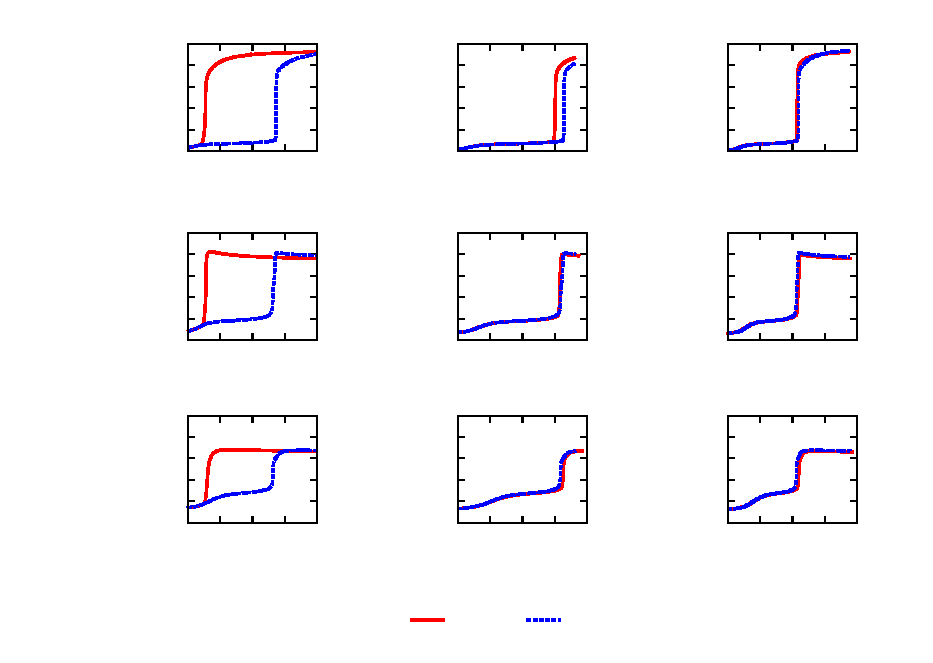
\includegraphics{ch-dynamics/LFA_V}}%
    \gplfronttext
  \end{picture}%
\endgroup
}
  \normalsize
  \vspace{-0.2in}
  \caption{Comparison between CFD and LFA results.}
  \label{fig:LFA_V}
\end{figure}

\subsection{Autoignition and flame interaction}

As shown by LFA, under some conditions, inhomogeneous autoignition and premixed flame propagation both contribute to flame stabilization, resulting in a multimode stabilized regime.  Furthermore, the interaction between autoignition and flame propagation is tightly coupled.  If the thermal structure is mainly \emph{kinetically} stabilized, heat and radicals generated by autoignition will modify the  downstream thermal and chemical environment and thus the local flame speed.  On the contrary, if stabilization is mainly \emph{kinematic} in nature then heat and radicals generated by the flame can back diffuse upstream, modifying the reactivity upstream.  

To demonstrate these complex interactions and understand the transition between \emph{kinetic} and \emph{kinematic} stabilization mechanisms, the LFA results for the $2.4$ m/s case were further analyzed.  As shown in Fig.~\ref{fig:LFA_V}, if there was a \emph{kinetically} stabilized inhomogeneous autoignition front, this front would stabilize further downstream than the \emph{kinematically} stabilized flame front.  Although not shown, CEMA of these LFA solutions show the same evolution of the controlling chemistry as the $8.0$ m/s case.  In particular, the low-to-intermediate temperature hydrogen peroxide chain branching reaction dominates the transition to autoignition.  Therefore, the nature and the qualitative structures of the inhomogeneous autoignition fronts, as predicted by LFA in Fig.~\ref{fig:LFA_V} for the two lower inlet velocity cases, are essentially the same as the $8.0$ m/s case.  

A general description of the initiation of these multibrachial inhomogeneous autoignition fronts in all three cases is that, due to radical accumulation and heat release, the controlling chemistry shifts from low temperature chemistry, represented by CH$_3$OCH$_2$O$_2$ reactions, to hydrogen peroxide branching reactions.  At some mixture fractions, higher temperatures and more oxidizer supply enable the dominant chemistry to transition further to high temperature chemistry, as characterized by the H radical branching reaction.  As shown in Fig.~\ref{fig:1D_V}, there are double or triple heat release peaks, depending on the mixture fraction.  However, for all mixture fractions, these peaks correlate very well with the inflection points on the temperature profiles and peaks on the OH radical profiles.  Comparing them with the CH$_3$OCH$_2$O$_2$ radical profile, it is clear that low temperature chemistry results in the first peak of heat release profile and produces OH radicals.  Hydrogen peroxide accumulates until it decomposes at the second heat release peak and produces OH radicals through H$_2$O$_2$ + M $\Longleftrightarrow$ OH + OH + M.  At $Z_{\rm st}$ and $Z = 0.2$, there is a third heat release and OH radical peak, which is due to the H + O$_2$ $\Longleftrightarrow$ O + OH reaction.  At $Z_{\rm st}$, the second and third peaks appear to be much closer compared with those at $Z = 0.2$, probably due to higher temperature and more abundant oxidizer, such that the H radical chain branching reaction is activated earlier.  Due to the lack of oxidizer, the third peak is not observed at $Z = 0.3$.  

\begin{figure}
  \vspace{-1in}
  \centering
  \scriptsize
  % GNUPLOT: LaTeX picture with Postscript
\begingroup
  \makeatletter
  \providecommand\color[2][]{%
    \GenericError{(gnuplot) \space\space\space\@spaces}{%
      Package color not loaded in conjunction with
      terminal option `colourtext'%
    }{See the gnuplot documentation for explanation.%
    }{Either use 'blacktext' in gnuplot or load the package
      color.sty in LaTeX.}%
    \renewcommand\color[2][]{}%
  }%
  \providecommand\includegraphics[2][]{%
    \GenericError{(gnuplot) \space\space\space\@spaces}{%
      Package graphicx or graphics not loaded%
    }{See the gnuplot documentation for explanation.%
    }{The gnuplot epslatex terminal needs graphicx.sty or graphics.sty.}%
    \renewcommand\includegraphics[2][]{}%
  }%
  \providecommand\rotatebox[2]{#2}%
  \@ifundefined{ifGPcolor}{%
    \newif\ifGPcolor
    \GPcolortrue
  }{}%
  \@ifundefined{ifGPblacktext}{%
    \newif\ifGPblacktext
    \GPblacktexttrue
  }{}%
  % define a \g@addto@macro without @ in the name:
  \let\gplgaddtomacro\g@addto@macro
  % define empty templates for all commands taking text:
  \gdef\gplbacktext{}%
  \gdef\gplfronttext{}%
  \makeatother
  \ifGPblacktext
    % no textcolor at all
    \def\colorrgb#1{}%
    \def\colorgray#1{}%
  \else
    % gray or color?
    \ifGPcolor
      \def\colorrgb#1{\color[rgb]{#1}}%
      \def\colorgray#1{\color[gray]{#1}}%
      \expandafter\def\csname LTw\endcsname{\color{white}}%
      \expandafter\def\csname LTb\endcsname{\color{black}}%
      \expandafter\def\csname LTa\endcsname{\color{black}}%
      \expandafter\def\csname LT0\endcsname{\color[rgb]{1,0,0}}%
      \expandafter\def\csname LT1\endcsname{\color[rgb]{0,1,0}}%
      \expandafter\def\csname LT2\endcsname{\color[rgb]{0,0,1}}%
      \expandafter\def\csname LT3\endcsname{\color[rgb]{1,0,1}}%
      \expandafter\def\csname LT4\endcsname{\color[rgb]{0,1,1}}%
      \expandafter\def\csname LT5\endcsname{\color[rgb]{1,1,0}}%
      \expandafter\def\csname LT6\endcsname{\color[rgb]{0,0,0}}%
      \expandafter\def\csname LT7\endcsname{\color[rgb]{1,0.3,0}}%
      \expandafter\def\csname LT8\endcsname{\color[rgb]{0.5,0.5,0.5}}%
    \else
      % gray
      \def\colorrgb#1{\color{black}}%
      \def\colorgray#1{\color[gray]{#1}}%
      \expandafter\def\csname LTw\endcsname{\color{white}}%
      \expandafter\def\csname LTb\endcsname{\color{black}}%
      \expandafter\def\csname LTa\endcsname{\color{black}}%
      \expandafter\def\csname LT0\endcsname{\color{black}}%
      \expandafter\def\csname LT1\endcsname{\color{black}}%
      \expandafter\def\csname LT2\endcsname{\color{black}}%
      \expandafter\def\csname LT3\endcsname{\color{black}}%
      \expandafter\def\csname LT4\endcsname{\color{black}}%
      \expandafter\def\csname LT5\endcsname{\color{black}}%
      \expandafter\def\csname LT6\endcsname{\color{black}}%
      \expandafter\def\csname LT7\endcsname{\color{black}}%
      \expandafter\def\csname LT8\endcsname{\color{black}}%
    \fi
  \fi
  \setlength{\unitlength}{0.0500bp}%
  \begin{picture}(5760.00,2520.00)%
    \gplgaddtomacro\gplbacktext{%
      \csname LTb\endcsname%
      \put(1342,440){\makebox(0,0)[r]{\strut{}1.0e+08}}%
      \put(1342,1045){\makebox(0,0)[r]{\strut{}1.0e+10}}%
      \put(1342,1651){\makebox(0,0)[r]{\strut{}1.0e+12}}%
      \put(1342,2256){\makebox(0,0)[r]{\strut{}1.0e+14}}%
      \put(1474,220){\makebox(0,0){\strut{} 0}}%
      \put(2446,220){\makebox(0,0){\strut{} 0.3}}%
      \put(3419,220){\makebox(0,0){\strut{} 0.6}}%
      \put(4391,220){\makebox(0,0){\strut{} 0.9}}%
      \put(5363,220){\makebox(0,0){\strut{} 1.2}}%
      \put(176,1348){\rotatebox{-270}{\makebox(0,0){\strut{}\vspace{-28pt}$HRR$ [J/m$^3$-s]}}}%
    }%
    \gplgaddtomacro\gplfronttext{%
      \csname LTb\endcsname%
      \put(2530,2083){\makebox(0,0)[r]{\strut{}$Z_{\rm st}$}}%
      \csname LTb\endcsname%
      \put(2530,1863){\makebox(0,0)[r]{\strut{}$Z = 0.2$}}%
      \csname LTb\endcsname%
      \put(2530,1643){\makebox(0,0)[r]{\strut{}$Z = 0.3$}}%
    }%
    \gplbacktext
    \put(0,0){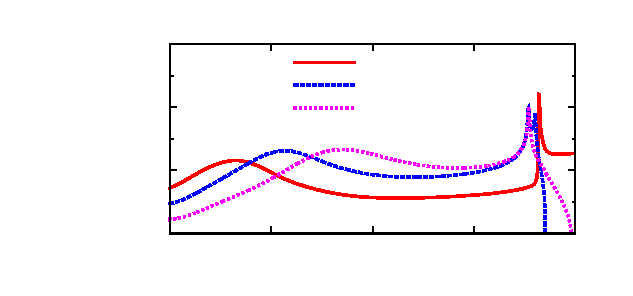
\includegraphics{1D_V_HRR}}%
    \gplfronttext
  \end{picture}%
\endgroup

%  \vspace{-0.3in}
  % GNUPLOT: LaTeX picture with Postscript
\begingroup
  \makeatletter
  \providecommand\color[2][]{%
    \GenericError{(gnuplot) \space\space\space\@spaces}{%
      Package color not loaded in conjunction with
      terminal option `colourtext'%
    }{See the gnuplot documentation for explanation.%
    }{Either use 'blacktext' in gnuplot or load the package
      color.sty in LaTeX.}%
    \renewcommand\color[2][]{}%
  }%
  \providecommand\includegraphics[2][]{%
    \GenericError{(gnuplot) \space\space\space\@spaces}{%
      Package graphicx or graphics not loaded%
    }{See the gnuplot documentation for explanation.%
    }{The gnuplot epslatex terminal needs graphicx.sty or graphics.sty.}%
    \renewcommand\includegraphics[2][]{}%
  }%
  \providecommand\rotatebox[2]{#2}%
  \@ifundefined{ifGPcolor}{%
    \newif\ifGPcolor
    \GPcolortrue
  }{}%
  \@ifundefined{ifGPblacktext}{%
    \newif\ifGPblacktext
    \GPblacktexttrue
  }{}%
  % define a \g@addto@macro without @ in the name:
  \let\gplgaddtomacro\g@addto@macro
  % define empty templates for all commands taking text:
  \gdef\gplbacktext{}%
  \gdef\gplfronttext{}%
  \makeatother
  \ifGPblacktext
    % no textcolor at all
    \def\colorrgb#1{}%
    \def\colorgray#1{}%
  \else
    % gray or color?
    \ifGPcolor
      \def\colorrgb#1{\color[rgb]{#1}}%
      \def\colorgray#1{\color[gray]{#1}}%
      \expandafter\def\csname LTw\endcsname{\color{white}}%
      \expandafter\def\csname LTb\endcsname{\color{black}}%
      \expandafter\def\csname LTa\endcsname{\color{black}}%
      \expandafter\def\csname LT0\endcsname{\color[rgb]{1,0,0}}%
      \expandafter\def\csname LT1\endcsname{\color[rgb]{0,1,0}}%
      \expandafter\def\csname LT2\endcsname{\color[rgb]{0,0,1}}%
      \expandafter\def\csname LT3\endcsname{\color[rgb]{1,0,1}}%
      \expandafter\def\csname LT4\endcsname{\color[rgb]{0,1,1}}%
      \expandafter\def\csname LT5\endcsname{\color[rgb]{1,1,0}}%
      \expandafter\def\csname LT6\endcsname{\color[rgb]{0,0,0}}%
      \expandafter\def\csname LT7\endcsname{\color[rgb]{1,0.3,0}}%
      \expandafter\def\csname LT8\endcsname{\color[rgb]{0.5,0.5,0.5}}%
    \else
      % gray
      \def\colorrgb#1{\color{black}}%
      \def\colorgray#1{\color[gray]{#1}}%
      \expandafter\def\csname LTw\endcsname{\color{white}}%
      \expandafter\def\csname LTb\endcsname{\color{black}}%
      \expandafter\def\csname LTa\endcsname{\color{black}}%
      \expandafter\def\csname LT0\endcsname{\color{black}}%
      \expandafter\def\csname LT1\endcsname{\color{black}}%
      \expandafter\def\csname LT2\endcsname{\color{black}}%
      \expandafter\def\csname LT3\endcsname{\color{black}}%
      \expandafter\def\csname LT4\endcsname{\color{black}}%
      \expandafter\def\csname LT5\endcsname{\color{black}}%
      \expandafter\def\csname LT6\endcsname{\color{black}}%
      \expandafter\def\csname LT7\endcsname{\color{black}}%
      \expandafter\def\csname LT8\endcsname{\color{black}}%
    \fi
  \fi
  \setlength{\unitlength}{0.0500bp}%
  \begin{picture}(5760.00,2520.00)%
    \gplgaddtomacro\gplbacktext{%
      \csname LTb\endcsname%
      \put(1342,440){\makebox(0,0)[r]{\strut{}5.0e+02}}%
      \put(1342,1045){\makebox(0,0)[r]{\strut{}1.2e+03}}%
      \put(1342,1651){\makebox(0,0)[r]{\strut{}1.9e+03}}%
      \put(1342,2256){\makebox(0,0)[r]{\strut{}2.6e+03}}%
      \put(1474,220){\makebox(0,0){\strut{} 0}}%
      \put(2446,220){\makebox(0,0){\strut{} 0.3}}%
      \put(3419,220){\makebox(0,0){\strut{} 0.6}}%
      \put(4391,220){\makebox(0,0){\strut{} 0.9}}%
      \put(5363,220){\makebox(0,0){\strut{} 1.2}}%
      \put(176,1348){\rotatebox{-270}{\makebox(0,0){\strut{}\vspace{-28pt}$T$ [K]}}}%
    }%
    \gplgaddtomacro\gplfronttext{%
      \csname LTb\endcsname%
      \put(2530,2083){\makebox(0,0)[r]{\strut{}$Z_{\rm st}$}}%
      \csname LTb\endcsname%
      \put(2530,1863){\makebox(0,0)[r]{\strut{}$Z = 0.2$}}%
      \csname LTb\endcsname%
      \put(2530,1643){\makebox(0,0)[r]{\strut{}$Z = 0.3$}}%
    }%
    \gplbacktext
    \put(0,0){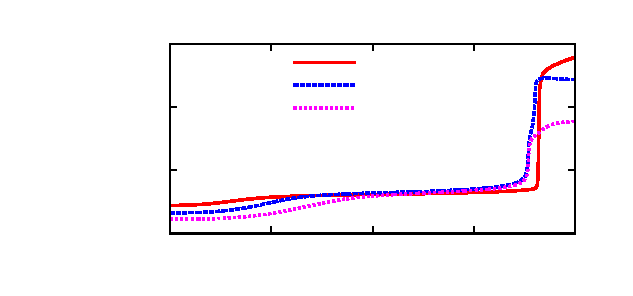
\includegraphics{ch-dynamics/1D_V_T}}%
    \gplfronttext
  \end{picture}%
\endgroup

%  \vspace{-0.3in}
  % GNUPLOT: LaTeX picture with Postscript
\begingroup
  \makeatletter
  \providecommand\color[2][]{%
    \GenericError{(gnuplot) \space\space\space\@spaces}{%
      Package color not loaded in conjunction with
      terminal option `colourtext'%
    }{See the gnuplot documentation for explanation.%
    }{Either use 'blacktext' in gnuplot or load the package
      color.sty in LaTeX.}%
    \renewcommand\color[2][]{}%
  }%
  \providecommand\includegraphics[2][]{%
    \GenericError{(gnuplot) \space\space\space\@spaces}{%
      Package graphicx or graphics not loaded%
    }{See the gnuplot documentation for explanation.%
    }{The gnuplot epslatex terminal needs graphicx.sty or graphics.sty.}%
    \renewcommand\includegraphics[2][]{}%
  }%
  \providecommand\rotatebox[2]{#2}%
  \@ifundefined{ifGPcolor}{%
    \newif\ifGPcolor
    \GPcolortrue
  }{}%
  \@ifundefined{ifGPblacktext}{%
    \newif\ifGPblacktext
    \GPblacktexttrue
  }{}%
  % define a \g@addto@macro without @ in the name:
  \let\gplgaddtomacro\g@addto@macro
  % define empty templates for all commands taking text:
  \gdef\gplbacktext{}%
  \gdef\gplfronttext{}%
  \makeatother
  \ifGPblacktext
    % no textcolor at all
    \def\colorrgb#1{}%
    \def\colorgray#1{}%
  \else
    % gray or color?
    \ifGPcolor
      \def\colorrgb#1{\color[rgb]{#1}}%
      \def\colorgray#1{\color[gray]{#1}}%
      \expandafter\def\csname LTw\endcsname{\color{white}}%
      \expandafter\def\csname LTb\endcsname{\color{black}}%
      \expandafter\def\csname LTa\endcsname{\color{black}}%
      \expandafter\def\csname LT0\endcsname{\color[rgb]{1,0,0}}%
      \expandafter\def\csname LT1\endcsname{\color[rgb]{0,1,0}}%
      \expandafter\def\csname LT2\endcsname{\color[rgb]{0,0,1}}%
      \expandafter\def\csname LT3\endcsname{\color[rgb]{1,0,1}}%
      \expandafter\def\csname LT4\endcsname{\color[rgb]{0,1,1}}%
      \expandafter\def\csname LT5\endcsname{\color[rgb]{1,1,0}}%
      \expandafter\def\csname LT6\endcsname{\color[rgb]{0,0,0}}%
      \expandafter\def\csname LT7\endcsname{\color[rgb]{1,0.3,0}}%
      \expandafter\def\csname LT8\endcsname{\color[rgb]{0.5,0.5,0.5}}%
    \else
      % gray
      \def\colorrgb#1{\color{black}}%
      \def\colorgray#1{\color[gray]{#1}}%
      \expandafter\def\csname LTw\endcsname{\color{white}}%
      \expandafter\def\csname LTb\endcsname{\color{black}}%
      \expandafter\def\csname LTa\endcsname{\color{black}}%
      \expandafter\def\csname LT0\endcsname{\color{black}}%
      \expandafter\def\csname LT1\endcsname{\color{black}}%
      \expandafter\def\csname LT2\endcsname{\color{black}}%
      \expandafter\def\csname LT3\endcsname{\color{black}}%
      \expandafter\def\csname LT4\endcsname{\color{black}}%
      \expandafter\def\csname LT5\endcsname{\color{black}}%
      \expandafter\def\csname LT6\endcsname{\color{black}}%
      \expandafter\def\csname LT7\endcsname{\color{black}}%
      \expandafter\def\csname LT8\endcsname{\color{black}}%
    \fi
  \fi
  \setlength{\unitlength}{0.0500bp}%
  \begin{picture}(5760.00,2520.00)%
    \gplgaddtomacro\gplbacktext{%
      \csname LTb\endcsname%
      \put(1342,440){\makebox(0,0)[r]{\strut{}1.0e-08}}%
      \put(1342,1045){\makebox(0,0)[r]{\strut{}1.0e-06}}%
      \put(1342,1651){\makebox(0,0)[r]{\strut{}1.0e-04}}%
      \put(1342,2256){\makebox(0,0)[r]{\strut{}1.0e-02}}%
      \put(1474,220){\makebox(0,0){\strut{} 0}}%
      \put(2446,220){\makebox(0,0){\strut{} 0.3}}%
      \put(3419,220){\makebox(0,0){\strut{} 0.6}}%
      \put(4391,220){\makebox(0,0){\strut{} 0.9}}%
      \put(5363,220){\makebox(0,0){\strut{} 1.2}}%
      \put(176,1348){\rotatebox{-270}{\makebox(0,0){\strut{}\vspace{-28pt}OH Mass Fraction}}}%
    }%
    \gplgaddtomacro\gplfronttext{%
      \csname LTb\endcsname%
      \put(2530,2083){\makebox(0,0)[r]{\strut{}$Z_{\rm st}$}}%
      \csname LTb\endcsname%
      \put(2530,1863){\makebox(0,0)[r]{\strut{}$Z = 0.2$}}%
      \csname LTb\endcsname%
      \put(2530,1643){\makebox(0,0)[r]{\strut{}$Z = 0.3$}}%
    }%
    \gplbacktext
    \put(0,0){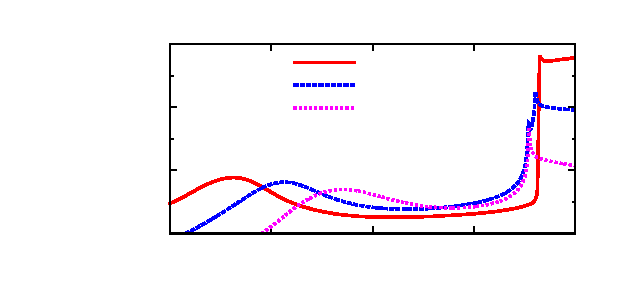
\includegraphics{1D_V_OH}}%
    \gplfronttext
  \end{picture}%
\endgroup

%  \vspace{-0.3in}
  % GNUPLOT: LaTeX picture with Postscript
\begingroup
  \makeatletter
  \providecommand\color[2][]{%
    \GenericError{(gnuplot) \space\space\space\@spaces}{%
      Package color not loaded in conjunction with
      terminal option `colourtext'%
    }{See the gnuplot documentation for explanation.%
    }{Either use 'blacktext' in gnuplot or load the package
      color.sty in LaTeX.}%
    \renewcommand\color[2][]{}%
  }%
  \providecommand\includegraphics[2][]{%
    \GenericError{(gnuplot) \space\space\space\@spaces}{%
      Package graphicx or graphics not loaded%
    }{See the gnuplot documentation for explanation.%
    }{The gnuplot epslatex terminal needs graphicx.sty or graphics.sty.}%
    \renewcommand\includegraphics[2][]{}%
  }%
  \providecommand\rotatebox[2]{#2}%
  \@ifundefined{ifGPcolor}{%
    \newif\ifGPcolor
    \GPcolortrue
  }{}%
  \@ifundefined{ifGPblacktext}{%
    \newif\ifGPblacktext
    \GPblacktexttrue
  }{}%
  % define a \g@addto@macro without @ in the name:
  \let\gplgaddtomacro\g@addto@macro
  % define empty templates for all commands taking text:
  \gdef\gplbacktext{}%
  \gdef\gplfronttext{}%
  \makeatother
  \ifGPblacktext
    % no textcolor at all
    \def\colorrgb#1{}%
    \def\colorgray#1{}%
  \else
    % gray or color?
    \ifGPcolor
      \def\colorrgb#1{\color[rgb]{#1}}%
      \def\colorgray#1{\color[gray]{#1}}%
      \expandafter\def\csname LTw\endcsname{\color{white}}%
      \expandafter\def\csname LTb\endcsname{\color{black}}%
      \expandafter\def\csname LTa\endcsname{\color{black}}%
      \expandafter\def\csname LT0\endcsname{\color[rgb]{1,0,0}}%
      \expandafter\def\csname LT1\endcsname{\color[rgb]{0,1,0}}%
      \expandafter\def\csname LT2\endcsname{\color[rgb]{0,0,1}}%
      \expandafter\def\csname LT3\endcsname{\color[rgb]{1,0,1}}%
      \expandafter\def\csname LT4\endcsname{\color[rgb]{0,1,1}}%
      \expandafter\def\csname LT5\endcsname{\color[rgb]{1,1,0}}%
      \expandafter\def\csname LT6\endcsname{\color[rgb]{0,0,0}}%
      \expandafter\def\csname LT7\endcsname{\color[rgb]{1,0.3,0}}%
      \expandafter\def\csname LT8\endcsname{\color[rgb]{0.5,0.5,0.5}}%
    \else
      % gray
      \def\colorrgb#1{\color{black}}%
      \def\colorgray#1{\color[gray]{#1}}%
      \expandafter\def\csname LTw\endcsname{\color{white}}%
      \expandafter\def\csname LTb\endcsname{\color{black}}%
      \expandafter\def\csname LTa\endcsname{\color{black}}%
      \expandafter\def\csname LT0\endcsname{\color{black}}%
      \expandafter\def\csname LT1\endcsname{\color{black}}%
      \expandafter\def\csname LT2\endcsname{\color{black}}%
      \expandafter\def\csname LT3\endcsname{\color{black}}%
      \expandafter\def\csname LT4\endcsname{\color{black}}%
      \expandafter\def\csname LT5\endcsname{\color{black}}%
      \expandafter\def\csname LT6\endcsname{\color{black}}%
      \expandafter\def\csname LT7\endcsname{\color{black}}%
      \expandafter\def\csname LT8\endcsname{\color{black}}%
    \fi
  \fi
  \setlength{\unitlength}{0.0500bp}%
  \begin{picture}(5760.00,2520.00)%
    \gplgaddtomacro\gplbacktext{%
      \csname LTb\endcsname%
      \put(1342,440){\makebox(0,0)[r]{\strut{}1.0e-08}}%
      \put(1342,1045){\makebox(0,0)[r]{\strut{}1.0e-06}}%
      \put(1342,1651){\makebox(0,0)[r]{\strut{}1.0e-04}}%
      \put(1342,2256){\makebox(0,0)[r]{\strut{}1.0e-02}}%
      \put(1474,220){\makebox(0,0){\strut{} 0}}%
      \put(2446,220){\makebox(0,0){\strut{} 0.3}}%
      \put(3419,220){\makebox(0,0){\strut{} 0.6}}%
      \put(4391,220){\makebox(0,0){\strut{} 0.9}}%
      \put(5363,220){\makebox(0,0){\strut{} 1.2}}%
      \put(176,1348){\rotatebox{-270}{\makebox(0,0){\strut{}\vspace{-28pt}CH$_3$OCH$_2$O$_2$ Mass Fraction}}}%
    }%
    \gplgaddtomacro\gplfronttext{%
      \csname LTb\endcsname%
      \put(2530,1053){\makebox(0,0)[r]{\strut{}$Z_{\rm st}$}}%
      \csname LTb\endcsname%
      \put(2530,833){\makebox(0,0)[r]{\strut{}$Z = 0.2$}}%
      \csname LTb\endcsname%
      \put(2530,613){\makebox(0,0)[r]{\strut{}$Z = 0.3$}}%
    }%
    \gplbacktext
    \put(0,0){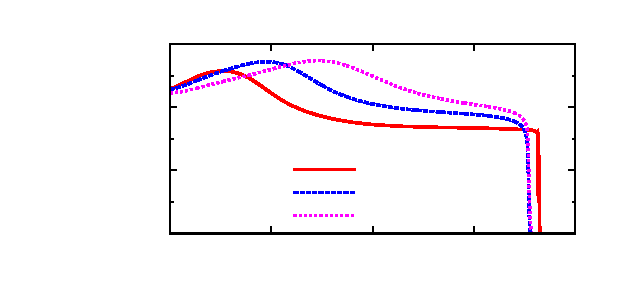
\includegraphics{1D_V_RO2}}%
    \gplfronttext
  \end{picture}%
\endgroup

%  \vspace{-0.3in}
  % GNUPLOT: LaTeX picture with Postscript
\begingroup
  \makeatletter
  \providecommand\color[2][]{%
    \GenericError{(gnuplot) \space\space\space\@spaces}{%
      Package color not loaded in conjunction with
      terminal option `colourtext'%
    }{See the gnuplot documentation for explanation.%
    }{Either use 'blacktext' in gnuplot or load the package
      color.sty in LaTeX.}%
    \renewcommand\color[2][]{}%
  }%
  \providecommand\includegraphics[2][]{%
    \GenericError{(gnuplot) \space\space\space\@spaces}{%
      Package graphicx or graphics not loaded%
    }{See the gnuplot documentation for explanation.%
    }{The gnuplot epslatex terminal needs graphicx.sty or graphics.sty.}%
    \renewcommand\includegraphics[2][]{}%
  }%
  \providecommand\rotatebox[2]{#2}%
  \@ifundefined{ifGPcolor}{%
    \newif\ifGPcolor
    \GPcolortrue
  }{}%
  \@ifundefined{ifGPblacktext}{%
    \newif\ifGPblacktext
    \GPblacktexttrue
  }{}%
  % define a \g@addto@macro without @ in the name:
  \let\gplgaddtomacro\g@addto@macro
  % define empty templates for all commands taking text:
  \gdef\gplbacktext{}%
  \gdef\gplfronttext{}%
  \makeatother
  \ifGPblacktext
    % no textcolor at all
    \def\colorrgb#1{}%
    \def\colorgray#1{}%
  \else
    % gray or color?
    \ifGPcolor
      \def\colorrgb#1{\color[rgb]{#1}}%
      \def\colorgray#1{\color[gray]{#1}}%
      \expandafter\def\csname LTw\endcsname{\color{white}}%
      \expandafter\def\csname LTb\endcsname{\color{black}}%
      \expandafter\def\csname LTa\endcsname{\color{black}}%
      \expandafter\def\csname LT0\endcsname{\color[rgb]{1,0,0}}%
      \expandafter\def\csname LT1\endcsname{\color[rgb]{0,1,0}}%
      \expandafter\def\csname LT2\endcsname{\color[rgb]{0,0,1}}%
      \expandafter\def\csname LT3\endcsname{\color[rgb]{1,0,1}}%
      \expandafter\def\csname LT4\endcsname{\color[rgb]{0,1,1}}%
      \expandafter\def\csname LT5\endcsname{\color[rgb]{1,1,0}}%
      \expandafter\def\csname LT6\endcsname{\color[rgb]{0,0,0}}%
      \expandafter\def\csname LT7\endcsname{\color[rgb]{1,0.3,0}}%
      \expandafter\def\csname LT8\endcsname{\color[rgb]{0.5,0.5,0.5}}%
    \else
      % gray
      \def\colorrgb#1{\color{black}}%
      \def\colorgray#1{\color[gray]{#1}}%
      \expandafter\def\csname LTw\endcsname{\color{white}}%
      \expandafter\def\csname LTb\endcsname{\color{black}}%
      \expandafter\def\csname LTa\endcsname{\color{black}}%
      \expandafter\def\csname LT0\endcsname{\color{black}}%
      \expandafter\def\csname LT1\endcsname{\color{black}}%
      \expandafter\def\csname LT2\endcsname{\color{black}}%
      \expandafter\def\csname LT3\endcsname{\color{black}}%
      \expandafter\def\csname LT4\endcsname{\color{black}}%
      \expandafter\def\csname LT5\endcsname{\color{black}}%
      \expandafter\def\csname LT6\endcsname{\color{black}}%
      \expandafter\def\csname LT7\endcsname{\color{black}}%
      \expandafter\def\csname LT8\endcsname{\color{black}}%
    \fi
  \fi
  \setlength{\unitlength}{0.0500bp}%
  \begin{picture}(5760.00,2520.00)%
    \gplgaddtomacro\gplbacktext{%
      \csname LTb\endcsname%
      \put(1342,704){\makebox(0,0)[r]{\strut{}1.0e-07}}%
      \put(1342,1221){\makebox(0,0)[r]{\strut{}1.0e-05}}%
      \put(1342,1739){\makebox(0,0)[r]{\strut{}1.0e-03}}%
      \put(1342,2256){\makebox(0,0)[r]{\strut{}1.0e-01}}%
      \put(1474,484){\makebox(0,0){\strut{} 0}}%
      \put(2446,484){\makebox(0,0){\strut{} 0.3}}%
      \put(3419,484){\makebox(0,0){\strut{} 0.6}}%
      \put(4391,484){\makebox(0,0){\strut{} 0.9}}%
      \put(5363,484){\makebox(0,0){\strut{} 1.2}}%
      \put(176,1480){\rotatebox{-270}{\makebox(0,0){\strut{}\vspace{-28pt}H$_2$O$_2$ Mass Fraction}}}%
      \put(3418,154){\makebox(0,0){\strut{}Time [ms]}}%
    }%
    \gplgaddtomacro\gplfronttext{%
      \csname LTb\endcsname%
      \put(2530,1317){\makebox(0,0)[r]{\strut{}$Z_{\rm st}$}}%
      \csname LTb\endcsname%
      \put(2530,1097){\makebox(0,0)[r]{\strut{}$Z = 0.2$}}%
      \csname LTb\endcsname%
      \put(2530,877){\makebox(0,0)[r]{\strut{}$Z = 0.3$}}%
    }%
    \gplbacktext
    \put(0,0){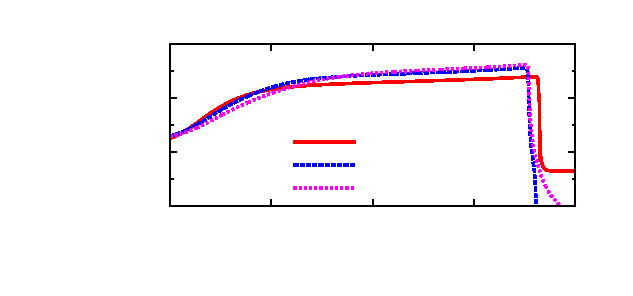
\includegraphics{1D_V_H2O2}}%
    \gplfronttext
  \end{picture}%
\endgroup

%  \vspace{-0.1875in}
  \normalsize
  \caption{LFA profiles along $Z_{\rm st}$, $Z = 0.2$, and $Z = 0.3$ of the $8.0$ m/s case.}
  \label{fig:1D_V}
\end{figure}

The multibrachial structure of the inhomogeneous autoignition front is due to the variation in ignition delay time at different mixture fractions.  As shown in Fig.~\ref{fig:HRR_V}, the stabilization point is determined based on the threshold value of heat release rate.  Therefore, the ignition delay time of inhomogeneous autoignition can be determined accordingly, which corresponds to the heat release rate peak that exceeds $10^{12}$ J/m$^3$-s.  For the $8.0$ m/s case shown in Fig.~\ref{fig:tau}, the mixture is autoignited first at $Z = 0.24$, which corresponds to the stabilization point in Fig.~\ref{fig:HRR_V}.  Although the first stage ignition delay time, defined by the first heat release peak through low temperature chemistry, increases monotonically as mixture fraction increases (temperature decreases), the overall ignition delay time reaches the shortest at $Z = 0.24$ due to the compensation of larger heat release after the first ignition stage~\cite{law12}, as shown in Fig.~\ref{fig:1D_V}.  As a consequence, although low temperature chemistry is not the dominant chemical pathway at the stabilization point for the \emph{kinetically} stabilized case, it still influences the location of the stabilization point through the mixture fraction dependent heat and radical accumulation upstream.    

\begin{figure}
  \vspace{-1in}
  \centering
  \scriptsize
  % GNUPLOT: LaTeX picture with Postscript
\begingroup
  \makeatletter
  \providecommand\color[2][]{%
    \GenericError{(gnuplot) \space\space\space\@spaces}{%
      Package color not loaded in conjunction with
      terminal option `colourtext'%
    }{See the gnuplot documentation for explanation.%
    }{Either use 'blacktext' in gnuplot or load the package
      color.sty in LaTeX.}%
    \renewcommand\color[2][]{}%
  }%
  \providecommand\includegraphics[2][]{%
    \GenericError{(gnuplot) \space\space\space\@spaces}{%
      Package graphicx or graphics not loaded%
    }{See the gnuplot documentation for explanation.%
    }{The gnuplot epslatex terminal needs graphicx.sty or graphics.sty.}%
    \renewcommand\includegraphics[2][]{}%
  }%
  \providecommand\rotatebox[2]{#2}%
  \@ifundefined{ifGPcolor}{%
    \newif\ifGPcolor
    \GPcolortrue
  }{}%
  \@ifundefined{ifGPblacktext}{%
    \newif\ifGPblacktext
    \GPblacktexttrue
  }{}%
  % define a \g@addto@macro without @ in the name:
  \let\gplgaddtomacro\g@addto@macro
  % define empty templates for all commands taking text:
  \gdef\gplbacktext{}%
  \gdef\gplfronttext{}%
  \makeatother
  \ifGPblacktext
    % no textcolor at all
    \def\colorrgb#1{}%
    \def\colorgray#1{}%
  \else
    % gray or color?
    \ifGPcolor
      \def\colorrgb#1{\color[rgb]{#1}}%
      \def\colorgray#1{\color[gray]{#1}}%
      \expandafter\def\csname LTw\endcsname{\color{white}}%
      \expandafter\def\csname LTb\endcsname{\color{black}}%
      \expandafter\def\csname LTa\endcsname{\color{black}}%
      \expandafter\def\csname LT0\endcsname{\color[rgb]{1,0,0}}%
      \expandafter\def\csname LT1\endcsname{\color[rgb]{0,1,0}}%
      \expandafter\def\csname LT2\endcsname{\color[rgb]{0,0,1}}%
      \expandafter\def\csname LT3\endcsname{\color[rgb]{1,0,1}}%
      \expandafter\def\csname LT4\endcsname{\color[rgb]{0,1,1}}%
      \expandafter\def\csname LT5\endcsname{\color[rgb]{1,1,0}}%
      \expandafter\def\csname LT6\endcsname{\color[rgb]{0,0,0}}%
      \expandafter\def\csname LT7\endcsname{\color[rgb]{1,0.3,0}}%
      \expandafter\def\csname LT8\endcsname{\color[rgb]{0.5,0.5,0.5}}%
    \else
      % gray
      \def\colorrgb#1{\color{black}}%
      \def\colorgray#1{\color[gray]{#1}}%
      \expandafter\def\csname LTw\endcsname{\color{white}}%
      \expandafter\def\csname LTb\endcsname{\color{black}}%
      \expandafter\def\csname LTa\endcsname{\color{black}}%
      \expandafter\def\csname LT0\endcsname{\color{black}}%
      \expandafter\def\csname LT1\endcsname{\color{black}}%
      \expandafter\def\csname LT2\endcsname{\color{black}}%
      \expandafter\def\csname LT3\endcsname{\color{black}}%
      \expandafter\def\csname LT4\endcsname{\color{black}}%
      \expandafter\def\csname LT5\endcsname{\color{black}}%
      \expandafter\def\csname LT6\endcsname{\color{black}}%
      \expandafter\def\csname LT7\endcsname{\color{black}}%
      \expandafter\def\csname LT8\endcsname{\color{black}}%
    \fi
  \fi
  \setlength{\unitlength}{0.0500bp}%
  \begin{picture}(3600.00,2520.00)%
    \gplgaddtomacro\gplbacktext{%
      \csname LTb\endcsname%
      \put(1078,704){\makebox(0,0)[r]{\strut{} 1.05}}%
      \put(1078,1221){\makebox(0,0)[r]{\strut{} 1.07}}%
      \put(1078,1739){\makebox(0,0)[r]{\strut{} 1.09}}%
      \put(1078,2256){\makebox(0,0)[r]{\strut{} 1.11}}%
      \put(1210,484){\makebox(0,0){\strut{} 0}}%
      \put(1708,484){\makebox(0,0){\strut{} 0.1}}%
      \put(2207,484){\makebox(0,0){\strut{} 0.2}}%
      \put(2705,484){\makebox(0,0){\strut{} 0.3}}%
      \put(3203,484){\makebox(0,0){\strut{} 0.4}}%
      \put(176,1480){\rotatebox{-270}{\makebox(0,0){\strut{}\vspace{-28pt}Iginition Delay [ms]}}}%
      \put(2206,154){\makebox(0,0){\strut{}Z}}%
    }%
    \gplgaddtomacro\gplfronttext{%
    }%
    \gplbacktext
    \put(0,0){
\includegraphics{tau_t}}%
    \gplfronttext
  \end{picture}%
\endgroup

%  \vspace{-0.3in}
  % GNUPLOT: LaTeX picture with Postscript
\begingroup
  \makeatletter
  \providecommand\color[2][]{%
    \GenericError{(gnuplot) \space\space\space\@spaces}{%
      Package color not loaded in conjunction with
      terminal option `colourtext'%
    }{See the gnuplot documentation for explanation.%
    }{Either use 'blacktext' in gnuplot or load the package
      color.sty in LaTeX.}%
    \renewcommand\color[2][]{}%
  }%
  \providecommand\includegraphics[2][]{%
    \GenericError{(gnuplot) \space\space\space\@spaces}{%
      Package graphicx or graphics not loaded%
    }{See the gnuplot documentation for explanation.%
    }{The gnuplot epslatex terminal needs graphicx.sty or graphics.sty.}%
    \renewcommand\includegraphics[2][]{}%
  }%
  \providecommand\rotatebox[2]{#2}%
  \@ifundefined{ifGPcolor}{%
    \newif\ifGPcolor
    \GPcolortrue
  }{}%
  \@ifundefined{ifGPblacktext}{%
    \newif\ifGPblacktext
    \GPblacktexttrue
  }{}%
  % define a \g@addto@macro without @ in the name:
  \let\gplgaddtomacro\g@addto@macro
  % define empty templates for all commands taking text:
  \gdef\gplbacktext{}%
  \gdef\gplfronttext{}%
  \makeatother
  \ifGPblacktext
    % no textcolor at all
    \def\colorrgb#1{}%
    \def\colorgray#1{}%
  \else
    % gray or color?
    \ifGPcolor
      \def\colorrgb#1{\color[rgb]{#1}}%
      \def\colorgray#1{\color[gray]{#1}}%
      \expandafter\def\csname LTw\endcsname{\color{white}}%
      \expandafter\def\csname LTb\endcsname{\color{black}}%
      \expandafter\def\csname LTa\endcsname{\color{black}}%
      \expandafter\def\csname LT0\endcsname{\color[rgb]{1,0,0}}%
      \expandafter\def\csname LT1\endcsname{\color[rgb]{0,1,0}}%
      \expandafter\def\csname LT2\endcsname{\color[rgb]{0,0,1}}%
      \expandafter\def\csname LT3\endcsname{\color[rgb]{1,0,1}}%
      \expandafter\def\csname LT4\endcsname{\color[rgb]{0,1,1}}%
      \expandafter\def\csname LT5\endcsname{\color[rgb]{1,1,0}}%
      \expandafter\def\csname LT6\endcsname{\color[rgb]{0,0,0}}%
      \expandafter\def\csname LT7\endcsname{\color[rgb]{1,0.3,0}}%
      \expandafter\def\csname LT8\endcsname{\color[rgb]{0.5,0.5,0.5}}%
    \else
      % gray
      \def\colorrgb#1{\color{black}}%
      \def\colorgray#1{\color[gray]{#1}}%
      \expandafter\def\csname LTw\endcsname{\color{white}}%
      \expandafter\def\csname LTb\endcsname{\color{black}}%
      \expandafter\def\csname LTa\endcsname{\color{black}}%
      \expandafter\def\csname LT0\endcsname{\color{black}}%
      \expandafter\def\csname LT1\endcsname{\color{black}}%
      \expandafter\def\csname LT2\endcsname{\color{black}}%
      \expandafter\def\csname LT3\endcsname{\color{black}}%
      \expandafter\def\csname LT4\endcsname{\color{black}}%
      \expandafter\def\csname LT5\endcsname{\color{black}}%
      \expandafter\def\csname LT6\endcsname{\color{black}}%
      \expandafter\def\csname LT7\endcsname{\color{black}}%
      \expandafter\def\csname LT8\endcsname{\color{black}}%
    \fi
  \fi
  \setlength{\unitlength}{0.0500bp}%
  \begin{picture}(3528.00,2520.00)%
    \gplgaddtomacro\gplbacktext{%
      \csname LTb\endcsname%
      \put(946,704){\makebox(0,0)[r]{\strut{} 0}}%
      \put(946,1221){\makebox(0,0)[r]{\strut{} 0.3}}%
      \put(946,1739){\makebox(0,0)[r]{\strut{} 0.6}}%
      \put(946,2256){\makebox(0,0)[r]{\strut{} 0.9}}%
      \put(1078,484){\makebox(0,0){\strut{} 0}}%
      \put(1591,484){\makebox(0,0){\strut{} 0.1}}%
      \put(2105,484){\makebox(0,0){\strut{} 0.2}}%
      \put(2618,484){\makebox(0,0){\strut{} 0.3}}%
      \put(3131,484){\makebox(0,0){\strut{} 0.4}}%
      \put(176,1480){\rotatebox{-270}{\makebox(0,0){\strut{}\vspace{-28pt}First Stage Ignition Delay [ms]}}}%
      \put(2104,154){\makebox(0,0){\strut{}Z}}%
    }%
    \gplgaddtomacro\gplfronttext{%
    }%
    \gplbacktext
    \put(0,0){
\includegraphics{ch-dynamics/tau_1}}%
    \gplfronttext
  \end{picture}%
\endgroup

%  \vspace{-0.3in}
  \normalsize
  \caption{LFA results on the mixture fraction dependent total and first stage ignition delay times of the $8.0$ m/s case.}
  \label{fig:tau}
\end{figure}              

However, although the cases in the current study are all initiated by inhomogeneous autoignition, the stabilization of the final structure depends on the dominant transport processes, which are influenced by the inlet velocities.  At $8.0$ m/s, heat and radical back diffusion from the autoignition front to upstream is not able to keep up with convection; therefore, the reacting front is \emph{kinetically} stabilized.  At $3.2$ m/s, as flow convection is weaker, diffusion processes become inherently important and couple with chemical reactions to induce a flame front propagating upstream.  However, the propagation speed of the flame varies with composition and temperature.  As a consequence, around $Z_{\rm st}$, where higher temperature and near-stoichiometric mixture composition enable higher local flame speed, the propagation of the reacting front balances the incoming flow velocity.  However, such a balance fails at richer mixture fractions where \emph{kinetic} stabilization dominates due to enhanced NTC-affected autoignition at richer mixture fractions as demonstrated in Fig.~\ref{fig:tau}.  At $2.4$ m/s, back diffusion is important at all mixture fractions such that the reacting front propagates upstream at the local flame speed, as determined by the local composition and temperature.  Due to the increased temperature and species stratification and the reduced thermal and radical accumulation from autoignition, the propagation speed of this reacting front is less influenced by inhomogeneous autoignition, as demonstrated with CEMA and LFA.  The structure of this \emph{kinematically} stabilized reacting front, which is generally tribrachial, is therefore determined by the variation of the local flame speed. 


       
%====================================================================
\section{Stabilization regime diagram}

The above sections have demonstrated the transport effects on the thermal and chemical structure of the lifted coflow flames as well as the stabilization mechanisms.  Combining these results with the chemical effects demonstrated by changing the coflow boundary temperature from our previous study~\cite{deng15}, a two-dimensional stabilization regime diagram is proposed, as shown in Fig.~\ref{fig:2D-regime}.   

\begin{figure}
  \centering
  \scriptsize
  \vspace{-0.1in}
  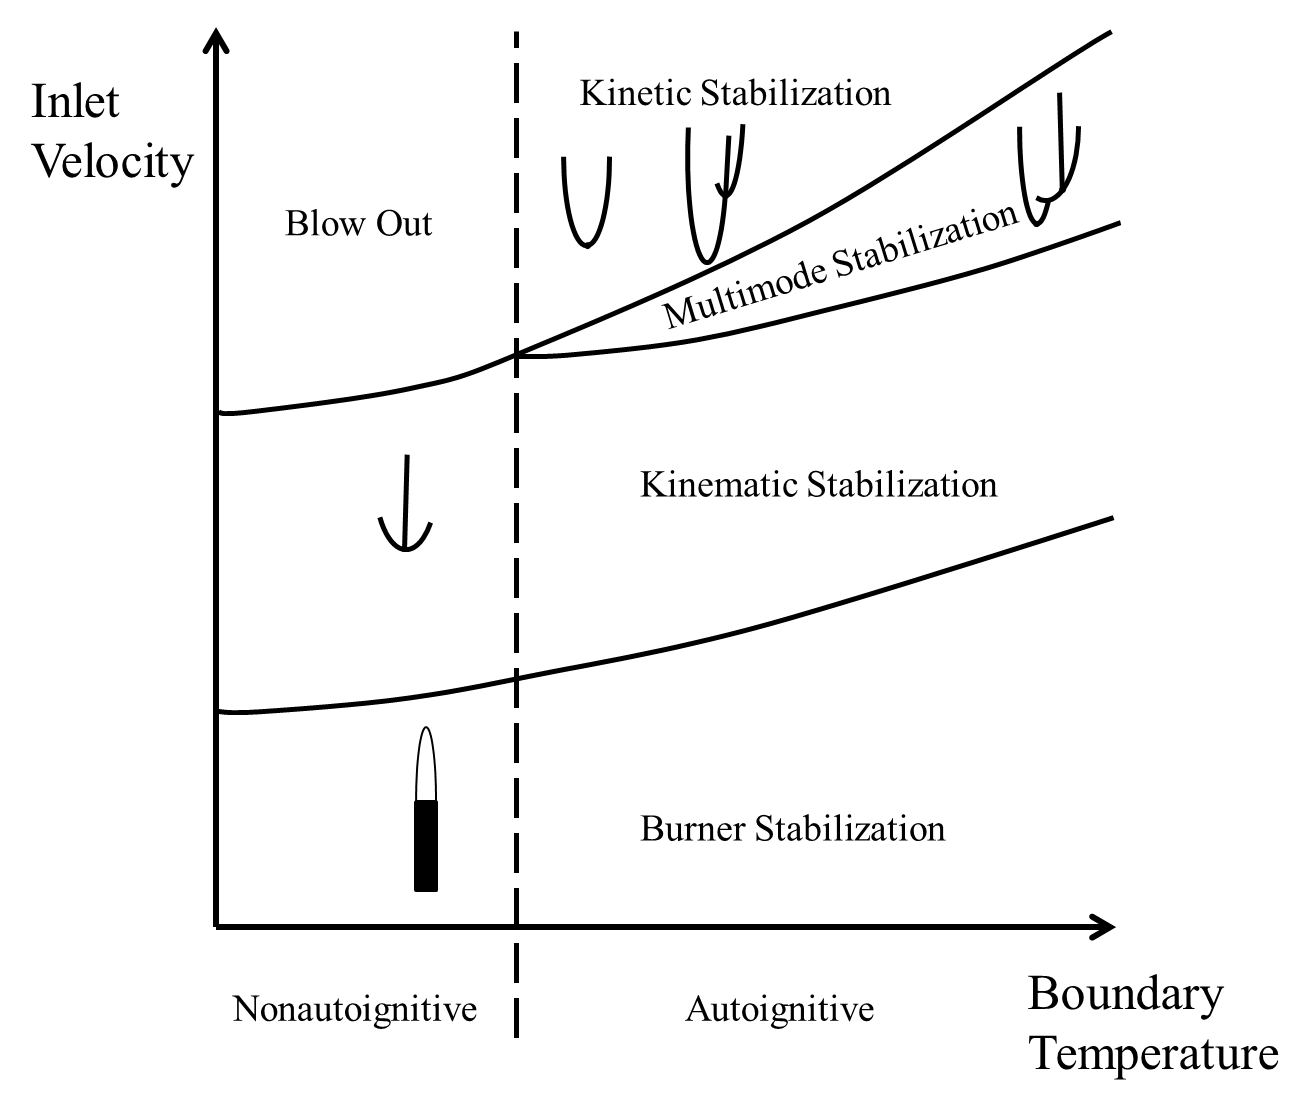
\includegraphics[width=1.0\textwidth]{2D-regime.png}
  \normalsize
  \vspace{-0.1in}
  \caption{A qualitative regime diagram for the stabilization mechanisms as the boundary temperature and inlet velocity vary. }
  \label{fig:2D-regime}
\end{figure}

Qualitatively, when the boundary temperature is not high enough to activate autoignition, the lifted flame appears as the classical triple flame and is \emph{kinematically} stabilized.  When the inlet velocity is below or above certain threshold values, the triple flame becomes attached to the burner or is blown out, respectively.  

As the boundary temperature is elevated enough to activate autoignition, increasing the inlet velocity while keeping constant boundary temperature, the flame stabilization mechanism transits from burner stabilization to a \emph{kinematic} balance between flame speed and incoming flow velocity, then to multimode stabilization influenced by both flame propagation and inhomogeneous autoignition, and finally to \emph {kinetic} stabilization governed by inhomogeneous autoignition.  It is expected that the crossover velocities between regimes increase with increasing boundary temperature because flame speed generally increases at higher temperature.  However, it is difficult to quantify these boundaries as local composition and temperature vary in the streamwise direction, and, therefore, the reference flame speed cannot be calculated based on the upstream boundary conditions.  Furthermore, local flame front curvature, cross-stream species stratification, and flow divergence approaching the flame front also modify the flame speed.  As a consequence, only a qualitative trend is demonstrated in Fig.~\ref{fig:2D-regime}.  

Similarly, if the boundary temperature increases at fixed inlet velocity, transition from blow out to burner stabilized regimes is achieved by moving horizontally across the regime diagram, which was discussed in our previous work~\cite{deng15}.     


%====================================================================

\section{Conclusions}

In the present work, axisymmetric two-dimensional laminar nonpremixed DME lifted coflow flames at elevated temperatures and pressures were computed.  Transport effects on the structure and stabilization mechanism were demonstrated by changing the inlet velocities while keeping the coflow boundary temperature constant.

The heat release rate profiles were examined to describe the thermal structure, and CEMA was used to demonstrate the evolution of the controlling chemistry.  Moreover, one-dimensional LFA that captures inhomogeneous autoignition was adopted to identify the dominant transport directions and therefore determine the dominant combustion mode and stabilization mechanism.

At $2.4$ m/s, the lifted flame appears to be the classical triple flame stabilized by the balance between the local flame speed and incoming flow velocity, and it is therefore characterized as \emph {kinematically} stabilized.  As the inlet velocity increases, such a balance cannot be achieved at certain mixture fractions.  Instead, inhomogeneous autoignition becomes the dominant combustion mode.  As a consequence, the multibrachial structure is stabilized by both premixed flame propagation and inhomogeneous autoignition and is characterized as multimode stabilized.  At $8.0$ m/s, the \emph{kinematic} balance cannot be achieved anywhere in the flow field due to lack of back diffusion.  A \emph{kinetically} stabilized inhomogeneous autoignition front is formed where diffusion processes along the mixture fraction iso-contours are negligible compared to the gradient direction.  In the \emph{kinetically} stabilized autoignition front, NTC chemistry plays an important role, dictating the stabilization point.  This point occurs at the mixture fraction with the shortest ignition delay time, which is a compromise of the first stage autoignition delay time and heat release from low temperature chemistry.  Conversely, the \emph{kinematically} stabilized flames are less affected by NTC chemistry, with only a minor effect on the local flame speed resulting from the upstream accumulation of heat and radicals.  Combined with the extended stabilization regimes demonstrated in our previous study~\cite{deng15}, an extended two-dimensional stabilization regime diagram was constructed, considering both transport (inlet velocity) and chemical (coflow boundary temperature) effects.  

\textcolor{Rv1}{This work represents a significant contribution to the understanding of nonpremixed flames at autoignitive conditions.  However, practical engines conditions are turbulent.  In such flows, the unsteady motion of eddies and enhanced temperature and species dissipation can strongly influence stabilization.  Therefore, further investigation is required to understand the role of turbulence in the stabilization of such flames and determine whether the stabilization mechanism is modified or not.} 

%====================================================================


\section*{Acknowledgments}
This research was supported in part by the Air Force Office of Scientific Research (AFOSR) under the technical management of Dr. Mitat Birkan.


\section*{References}
\bibliographystyle{elsarticle-num-CNF}
\bibliography{Jet2}

\renewcommand{\thefigure}{\arabic{figure}}
\renewcommand{\thetable}{\arabic{table}}




\end{document}





  
